\documentclass[]{article}
\usepackage{lmodern}
\usepackage{amssymb,amsmath}
\usepackage{ifxetex,ifluatex}
\usepackage{fixltx2e} % provides \textsubscript
\ifnum 0\ifxetex 1\fi\ifluatex 1\fi=0 % if pdftex
  \usepackage[T1]{fontenc}
  \usepackage[utf8]{inputenc}
\else % if luatex or xelatex
  \ifxetex
    \usepackage{mathspec}
  \else
    \usepackage{fontspec}
  \fi
  \defaultfontfeatures{Ligatures=TeX,Scale=MatchLowercase}
\fi
% use upquote if available, for straight quotes in verbatim environments
\IfFileExists{upquote.sty}{\usepackage{upquote}}{}
% use microtype if available
\IfFileExists{microtype.sty}{%
\usepackage{microtype}
\UseMicrotypeSet[protrusion]{basicmath} % disable protrusion for tt fonts
}{}
\usepackage[margin=1in]{geometry}
\usepackage{hyperref}
\hypersetup{unicode=true,
            pdftitle={Regression Analysis \#1},
            pdfauthor={Aleksander Molak},
            pdfborder={0 0 0},
            breaklinks=true}
\urlstyle{same}  % don't use monospace font for urls
\usepackage{color}
\usepackage{fancyvrb}
\newcommand{\VerbBar}{|}
\newcommand{\VERB}{\Verb[commandchars=\\\{\}]}
\DefineVerbatimEnvironment{Highlighting}{Verbatim}{commandchars=\\\{\}}
% Add ',fontsize=\small' for more characters per line
\usepackage{framed}
\definecolor{shadecolor}{RGB}{248,248,248}
\newenvironment{Shaded}{\begin{snugshade}}{\end{snugshade}}
\newcommand{\AlertTok}[1]{\textcolor[rgb]{0.94,0.16,0.16}{#1}}
\newcommand{\AnnotationTok}[1]{\textcolor[rgb]{0.56,0.35,0.01}{\textbf{\textit{#1}}}}
\newcommand{\AttributeTok}[1]{\textcolor[rgb]{0.77,0.63,0.00}{#1}}
\newcommand{\BaseNTok}[1]{\textcolor[rgb]{0.00,0.00,0.81}{#1}}
\newcommand{\BuiltInTok}[1]{#1}
\newcommand{\CharTok}[1]{\textcolor[rgb]{0.31,0.60,0.02}{#1}}
\newcommand{\CommentTok}[1]{\textcolor[rgb]{0.56,0.35,0.01}{\textit{#1}}}
\newcommand{\CommentVarTok}[1]{\textcolor[rgb]{0.56,0.35,0.01}{\textbf{\textit{#1}}}}
\newcommand{\ConstantTok}[1]{\textcolor[rgb]{0.00,0.00,0.00}{#1}}
\newcommand{\ControlFlowTok}[1]{\textcolor[rgb]{0.13,0.29,0.53}{\textbf{#1}}}
\newcommand{\DataTypeTok}[1]{\textcolor[rgb]{0.13,0.29,0.53}{#1}}
\newcommand{\DecValTok}[1]{\textcolor[rgb]{0.00,0.00,0.81}{#1}}
\newcommand{\DocumentationTok}[1]{\textcolor[rgb]{0.56,0.35,0.01}{\textbf{\textit{#1}}}}
\newcommand{\ErrorTok}[1]{\textcolor[rgb]{0.64,0.00,0.00}{\textbf{#1}}}
\newcommand{\ExtensionTok}[1]{#1}
\newcommand{\FloatTok}[1]{\textcolor[rgb]{0.00,0.00,0.81}{#1}}
\newcommand{\FunctionTok}[1]{\textcolor[rgb]{0.00,0.00,0.00}{#1}}
\newcommand{\ImportTok}[1]{#1}
\newcommand{\InformationTok}[1]{\textcolor[rgb]{0.56,0.35,0.01}{\textbf{\textit{#1}}}}
\newcommand{\KeywordTok}[1]{\textcolor[rgb]{0.13,0.29,0.53}{\textbf{#1}}}
\newcommand{\NormalTok}[1]{#1}
\newcommand{\OperatorTok}[1]{\textcolor[rgb]{0.81,0.36,0.00}{\textbf{#1}}}
\newcommand{\OtherTok}[1]{\textcolor[rgb]{0.56,0.35,0.01}{#1}}
\newcommand{\PreprocessorTok}[1]{\textcolor[rgb]{0.56,0.35,0.01}{\textit{#1}}}
\newcommand{\RegionMarkerTok}[1]{#1}
\newcommand{\SpecialCharTok}[1]{\textcolor[rgb]{0.00,0.00,0.00}{#1}}
\newcommand{\SpecialStringTok}[1]{\textcolor[rgb]{0.31,0.60,0.02}{#1}}
\newcommand{\StringTok}[1]{\textcolor[rgb]{0.31,0.60,0.02}{#1}}
\newcommand{\VariableTok}[1]{\textcolor[rgb]{0.00,0.00,0.00}{#1}}
\newcommand{\VerbatimStringTok}[1]{\textcolor[rgb]{0.31,0.60,0.02}{#1}}
\newcommand{\WarningTok}[1]{\textcolor[rgb]{0.56,0.35,0.01}{\textbf{\textit{#1}}}}
\usepackage{graphicx,grffile}
\makeatletter
\def\maxwidth{\ifdim\Gin@nat@width>\linewidth\linewidth\else\Gin@nat@width\fi}
\def\maxheight{\ifdim\Gin@nat@height>\textheight\textheight\else\Gin@nat@height\fi}
\makeatother
% Scale images if necessary, so that they will not overflow the page
% margins by default, and it is still possible to overwrite the defaults
% using explicit options in \includegraphics[width, height, ...]{}
\setkeys{Gin}{width=\maxwidth,height=\maxheight,keepaspectratio}
\IfFileExists{parskip.sty}{%
\usepackage{parskip}
}{% else
\setlength{\parindent}{0pt}
\setlength{\parskip}{6pt plus 2pt minus 1pt}
}
\setlength{\emergencystretch}{3em}  % prevent overfull lines
\providecommand{\tightlist}{%
  \setlength{\itemsep}{0pt}\setlength{\parskip}{0pt}}
\setcounter{secnumdepth}{0}
% Redefines (sub)paragraphs to behave more like sections
\ifx\paragraph\undefined\else
\let\oldparagraph\paragraph
\renewcommand{\paragraph}[1]{\oldparagraph{#1}\mbox{}}
\fi
\ifx\subparagraph\undefined\else
\let\oldsubparagraph\subparagraph
\renewcommand{\subparagraph}[1]{\oldsubparagraph{#1}\mbox{}}
\fi

%%% Use protect on footnotes to avoid problems with footnotes in titles
\let\rmarkdownfootnote\footnote%
\def\footnote{\protect\rmarkdownfootnote}

%%% Change title format to be more compact
\usepackage{titling}

% Create subtitle command for use in maketitle
\providecommand{\subtitle}[1]{
  \posttitle{
    \begin{center}\large#1\end{center}
    }
}

\setlength{\droptitle}{-2em}

  \title{Regression Analysis \#1}
    \pretitle{\vspace{\droptitle}\centering\huge}
  \posttitle{\par}
    \author{Aleksander Molak}
    \preauthor{\centering\large\emph}
  \postauthor{\par}
      \predate{\centering\large\emph}
  \postdate{\par}
    \date{November 28, 2019}


\begin{document}
\maketitle

\hypertarget{read-in-the-data}{%
\subsection{Read in the data}\label{read-in-the-data}}

\begin{Shaded}
\begin{Highlighting}[]
\NormalTok{data <-}\StringTok{ }\KeywordTok{read.spss}\NormalTok{(}\KeywordTok{file.path}\NormalTok{(path, data_file), }\DataTypeTok{to.data.frame =} \OtherTok{TRUE}\NormalTok{)}
\end{Highlighting}
\end{Shaded}

\begin{verbatim}
## re-encoding from UTF-8
\end{verbatim}

\hypertarget{exploratory-data-analysis}{%
\subsection{Exploratory data analysis}\label{exploratory-data-analysis}}

\begin{Shaded}
\begin{Highlighting}[]
\CommentTok{# Number of observations}
\KeywordTok{dim}\NormalTok{(data)[}\DecValTok{1}\NormalTok{]}
\end{Highlighting}
\end{Shaded}

\begin{verbatim}
## [1] 402
\end{verbatim}

\begin{Shaded}
\begin{Highlighting}[]
\KeywordTok{summary}\NormalTok{(data)}
\end{Highlighting}
\end{Shaded}

\begin{verbatim}
##      MONEY                         EDUC         SEX           FWI        
##  Min.   :  0.00   elementary         :102   female:202   Min.   :  0.00  
##  1st Qu.: 39.02   vocational         :100   male  :200   1st Qu.: 44.08  
##  Median : 52.95   general highschool : 49                Median : 77.49  
##  Mean   : 53.18   profiled highschool: 51                Mean   : 70.78  
##  3rd Qu.: 67.81   higher             :100                3rd Qu.:100.00  
##  Max.   :100.00                                          Max.   :250.00  
##        CI               AQ               II        
##  Min.   :  0.00   Min.   :  0.00   Min.   :  0.00  
##  1st Qu.: 34.25   1st Qu.: 38.35   1st Qu.: 37.95  
##  Median : 48.48   Median : 51.91   Median : 51.95  
##  Mean   : 49.63   Mean   : 52.38   Mean   : 52.18  
##  3rd Qu.: 62.69   3rd Qu.: 67.03   3rd Qu.: 66.47  
##  Max.   :100.00   Max.   :100.00   Max.   :100.00
\end{verbatim}

There's no missing data in the dataset.

There are two categorical variables in the dataset:

\begin{itemize}
\item
  \texttt{EDUC} with 5 levels
\item
  \texttt{SEX} with two levels
\end{itemize}

The latter can be simply encoded as a binary variable. The former needs
to be one-hot encoded.

\hypertarget{recode-clean-categorical-variables}{%
\subsection{Recode \& clean categorical
variables}\label{recode-clean-categorical-variables}}

We will use \texttt{male} as our reference point. It will be encoded as
\texttt{0}.

\begin{Shaded}
\begin{Highlighting}[]
\CommentTok{# Recode `SEX`}
\NormalTok{data}\OperatorTok{$}\NormalTok{SEX <-}\StringTok{ }\NormalTok{dplyr}\OperatorTok{::}\KeywordTok{recode}\NormalTok{(data}\OperatorTok{$}\NormalTok{SEX, }\DataTypeTok{male =} \DecValTok{0}\NormalTok{, }\DataTypeTok{female =} \DecValTok{1}\NormalTok{)}
\end{Highlighting}
\end{Shaded}

Education is a categorical variable - categories like
\texttt{general\ highschool} or \texttt{profiled\ highschool} do not
seem to be easily translatable to a interval or ratio scale. Let's
perform one-hot encoding for \texttt{EDUC}:

\begin{Shaded}
\begin{Highlighting}[]
\NormalTok{edu <-}\StringTok{ }\NormalTok{data }\OperatorTok\StringTok{ }\KeywordTok{select}\NormalTok{(EDUC)}
\NormalTok{edu_dummy <-}\StringTok{ }\NormalTok{dummies}\OperatorTok{::}\KeywordTok{dummy}\NormalTok{(edu}\OperatorTok{$}\NormalTok{EDUC, }\DataTypeTok{sep =} \StringTok{'_'}\NormalTok{)}
\end{Highlighting}
\end{Shaded}

\begin{verbatim}
## Warning in model.matrix.default(~x - 1, model.frame(~x - 1), contrasts =
## FALSE): non-list contrasts argument ignored
\end{verbatim}

\begin{Shaded}
\begin{Highlighting}[]
\NormalTok{data_ohe <-}\StringTok{ }\KeywordTok{cbind}\NormalTok{(data, edu_dummy)}
\end{Highlighting}
\end{Shaded}

Now, let's clean the data (remove the original \texttt{EDUC} column) and
pick our reference point for education. On one hand, I'd like to have a
reference somewhere in the middle, which could be a good basis for neat
interpretation. On the other hand, the middle category
(\texttt{general\ highscholool}) has less observations than many other
categories. Taking this into account, I'll choose \texttt{higher} as the
reference point, to minimize the coefficient standard errors.

\begin{Shaded}
\begin{Highlighting}[]
\NormalTok{data_ohe <-}\StringTok{ }\NormalTok{plyr}\OperatorTok{::}\KeywordTok{rename}\NormalTok{(data_ohe, }
                         \DataTypeTok{replace =} \KeywordTok{c}\NormalTok{(}\StringTok{'EDUC_profiled highschool'}\NormalTok{ =}\StringTok{ 'EDUC_profiled_highschool'}\NormalTok{,}
                                     \StringTok{'EDUC_general highschool'}\NormalTok{  =}\StringTok{ 'EDUC_general_highschool'}\NormalTok{))}
\end{Highlighting}
\end{Shaded}

\begin{verbatim}
## The following `from` values were not present in `x`: EDUC_profiled highschool, EDUC_general highschool
\end{verbatim}

\begin{Shaded}
\begin{Highlighting}[]
\CommentTok{# #### Knitr throws an error here: save the data to csv and re-read ####}
\CommentTok{# data_clean <- data_ohe %>% select(-c(EDUC))}
\CommentTok{# data_clean <- data_clean %>% select(-c(EDUC_higher))}
\CommentTok{# # }
\CommentTok{# write.csv(data_clean, file.path(path, 'data_clean.csv'), row.names = FALSE)}
\NormalTok{data_clean <-}\StringTok{ }\KeywordTok{read.csv}\NormalTok{(}\KeywordTok{file.path}\NormalTok{(path, }\StringTok{'data_clean.csv'}\NormalTok{))}
\end{Highlighting}
\end{Shaded}

\hypertarget{examine-numerical-variables}{%
\subsection{Examine numerical
variables}\label{examine-numerical-variables}}

\hypertarget{histograms}{%
\subsubsection{Histograms}\label{histograms}}

\begin{Shaded}
\begin{Highlighting}[]
\CommentTok{# Histogram of DV - MONEY}
\KeywordTok{ggplot}\NormalTok{(data_clean, }\KeywordTok{aes}\NormalTok{(MONEY)) }\OperatorTok{+}\StringTok{ }\KeywordTok{geom_histogram}\NormalTok{(}\DataTypeTok{bins=}\DecValTok{7}\NormalTok{, }\DataTypeTok{fill=}\NormalTok{color, }\DataTypeTok{alpha=}\NormalTok{.}\DecValTok{7}\NormalTok{) }\OperatorTok{+}\StringTok{ }
\StringTok{                           }\KeywordTok{xlab}\NormalTok{(}\StringTok{'Wage'}\NormalTok{) }\OperatorTok{+}\StringTok{ }
\StringTok{                           }\KeywordTok{ylab}\NormalTok{(}\StringTok{'Count'}\NormalTok{) }\OperatorTok{+}\StringTok{ }
\StringTok{                           }\KeywordTok{theme_minimal}\NormalTok{()}
\end{Highlighting}
\end{Shaded}

\begin{figure}

{\centering 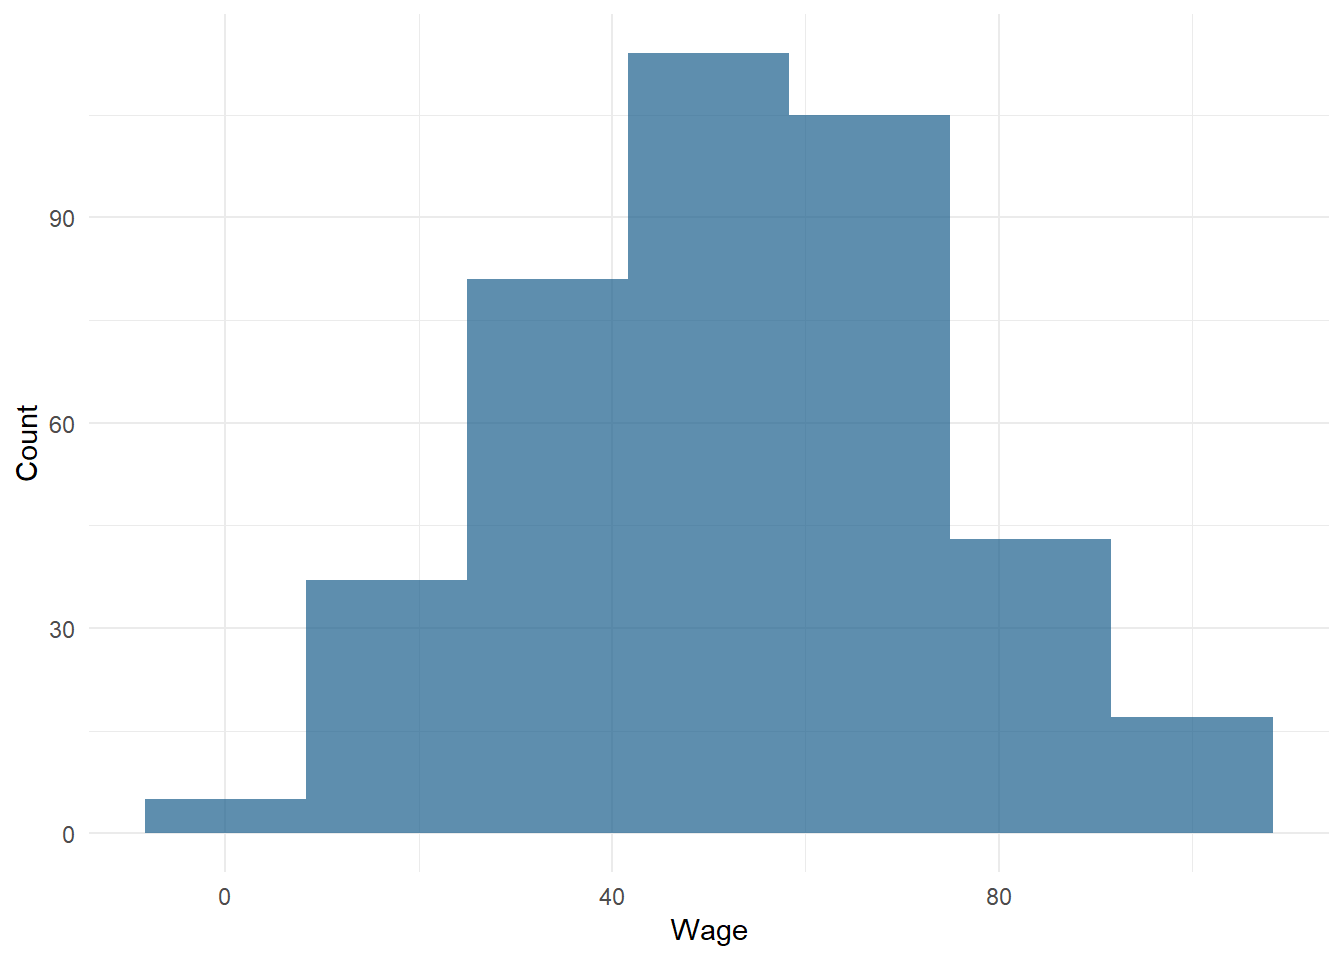
\includegraphics{regression_1_files/figure-latex/unnamed-chunk-9-1} 

}

\caption{Figure 1. Histogram: Wage}\label{fig:unnamed-chunk-9}
\end{figure}

\begin{Shaded}
\begin{Highlighting}[]
\CommentTok{# Histogram of DV - MONEY}
\KeywordTok{ggplot}\NormalTok{(data_clean, }\KeywordTok{aes}\NormalTok{(FWI)) }\OperatorTok{+}\StringTok{ }\KeywordTok{geom_histogram}\NormalTok{(}\DataTypeTok{bins=}\DecValTok{7}\NormalTok{, }\DataTypeTok{fill=}\NormalTok{color, }\DataTypeTok{alpha=}\NormalTok{.}\DecValTok{7}\NormalTok{) }\OperatorTok{+}\StringTok{ }
\StringTok{                           }\KeywordTok{xlab}\NormalTok{(}\StringTok{'Family Wealth Index'}\NormalTok{) }\OperatorTok{+}\StringTok{ }
\StringTok{                           }\KeywordTok{ylab}\NormalTok{(}\StringTok{'Count'}\NormalTok{) }\OperatorTok{+}\StringTok{ }
\StringTok{                           }\KeywordTok{theme_minimal}\NormalTok{()}
\end{Highlighting}
\end{Shaded}

\begin{figure}

{\centering 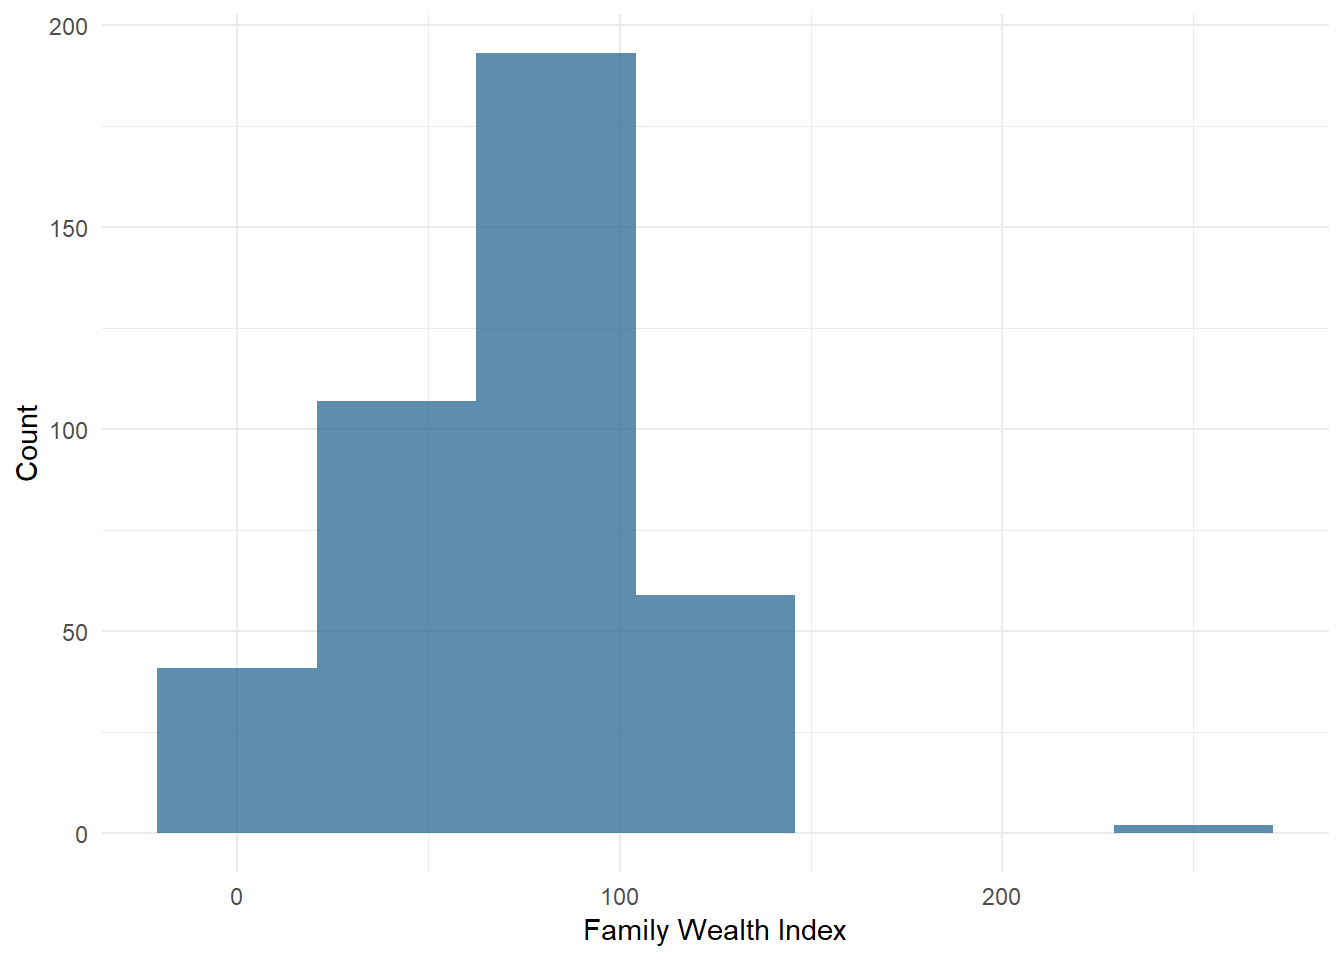
\includegraphics{regression_1_files/figure-latex/unnamed-chunk-10-1} 

}

\caption{Figure 2. Histogram: Family Wealth Index}\label{fig:unnamed-chunk-10}
\end{figure}

It seems that \texttt{FWI} contains a potentially problematic
observation(s). There is a small `bump' in the histogram around the
value of \texttt{250}. It's much higher than most other values for this
variable and much higher than \texttt{max} of other numerical variables
(\texttt{100}). Let's remeber about this and get back to this issue when
generating scatterplots.

\begin{Shaded}
\begin{Highlighting}[]
\CommentTok{# Histogram of DV - MONEY}
\KeywordTok{ggplot}\NormalTok{(data_clean, }\KeywordTok{aes}\NormalTok{(CI)) }\OperatorTok{+}\StringTok{ }\KeywordTok{geom_histogram}\NormalTok{(}\DataTypeTok{bins=}\DecValTok{7}\NormalTok{, }\DataTypeTok{fill=}\NormalTok{color, }\DataTypeTok{alpha=}\NormalTok{.}\DecValTok{7}\NormalTok{) }\OperatorTok{+}\StringTok{ }
\StringTok{                           }\KeywordTok{xlab}\NormalTok{(}\StringTok{'Competence Assessment Index'}\NormalTok{) }\OperatorTok{+}\StringTok{ }
\StringTok{                           }\KeywordTok{ylab}\NormalTok{(}\StringTok{'Count'}\NormalTok{) }\OperatorTok{+}\StringTok{ }
\StringTok{                           }\KeywordTok{theme_minimal}\NormalTok{()}
\end{Highlighting}
\end{Shaded}

\begin{figure}

{\centering 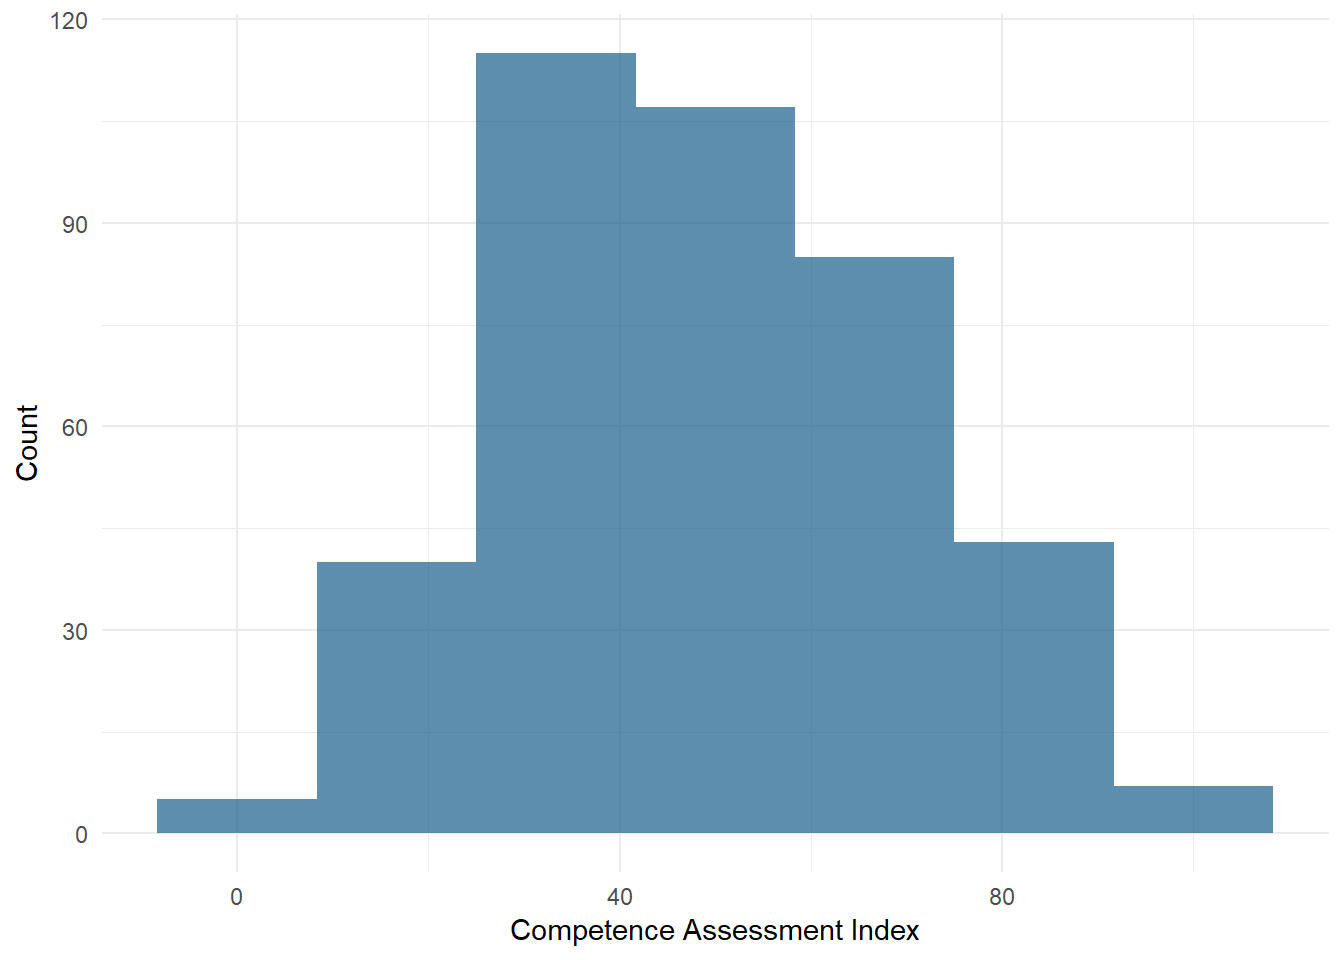
\includegraphics{regression_1_files/figure-latex/unnamed-chunk-11-1} 

}

\caption{Figure 4. Histogram: Competence Assessment Index}\label{fig:unnamed-chunk-11}
\end{figure}

\begin{Shaded}
\begin{Highlighting}[]
\CommentTok{# Histogram of DV - MONEY}
\KeywordTok{ggplot}\NormalTok{(data_clean, }\KeywordTok{aes}\NormalTok{(AQ)) }\OperatorTok{+}\StringTok{ }\KeywordTok{geom_histogram}\NormalTok{(}\DataTypeTok{bins=}\DecValTok{7}\NormalTok{, }\DataTypeTok{fill=}\NormalTok{color, }\DataTypeTok{alpha=}\NormalTok{.}\DecValTok{7}\NormalTok{) }\OperatorTok{+}\StringTok{ }
\StringTok{                           }\KeywordTok{xlab}\NormalTok{(}\StringTok{'Ambitions Questionnaire Score'}\NormalTok{) }\OperatorTok{+}\StringTok{ }
\StringTok{                           }\KeywordTok{ylab}\NormalTok{(}\StringTok{'Count'}\NormalTok{) }\OperatorTok{+}\StringTok{ }
\StringTok{                           }\KeywordTok{theme_minimal}\NormalTok{()}
\end{Highlighting}
\end{Shaded}

\begin{figure}

{\centering 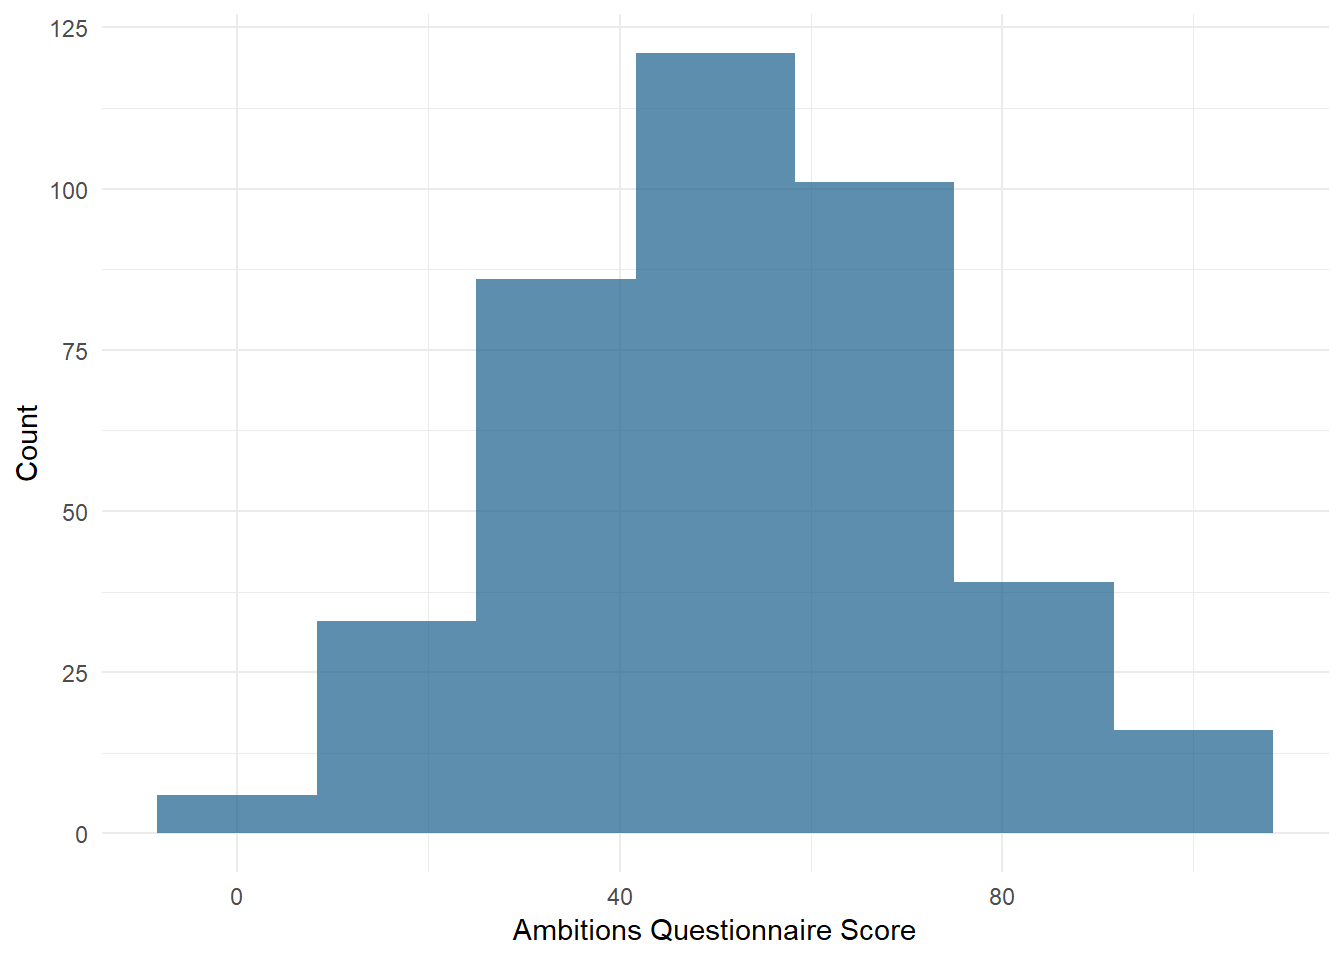
\includegraphics{regression_1_files/figure-latex/unnamed-chunk-12-1} 

}

\caption{Figure 5. Histogram: Ambitions Questionnaire Score}\label{fig:unnamed-chunk-12}
\end{figure}

\begin{Shaded}
\begin{Highlighting}[]
\CommentTok{# Histogram of DV - MONEY}
\KeywordTok{ggplot}\NormalTok{(data_clean, }\KeywordTok{aes}\NormalTok{(II)) }\OperatorTok{+}\StringTok{ }\KeywordTok{geom_histogram}\NormalTok{(}\DataTypeTok{bins=}\DecValTok{7}\NormalTok{, }\DataTypeTok{fill=}\NormalTok{color, }\DataTypeTok{alpha=}\NormalTok{.}\DecValTok{7}\NormalTok{) }\OperatorTok{+}\StringTok{ }
\StringTok{                           }\KeywordTok{xlab}\NormalTok{(}\StringTok{'Index of work involvement'}\NormalTok{) }\OperatorTok{+}\StringTok{ }
\StringTok{                           }\KeywordTok{ylab}\NormalTok{(}\StringTok{'Count'}\NormalTok{) }\OperatorTok{+}\StringTok{ }
\StringTok{                           }\KeywordTok{theme_minimal}\NormalTok{()}
\end{Highlighting}
\end{Shaded}

\begin{figure}

{\centering 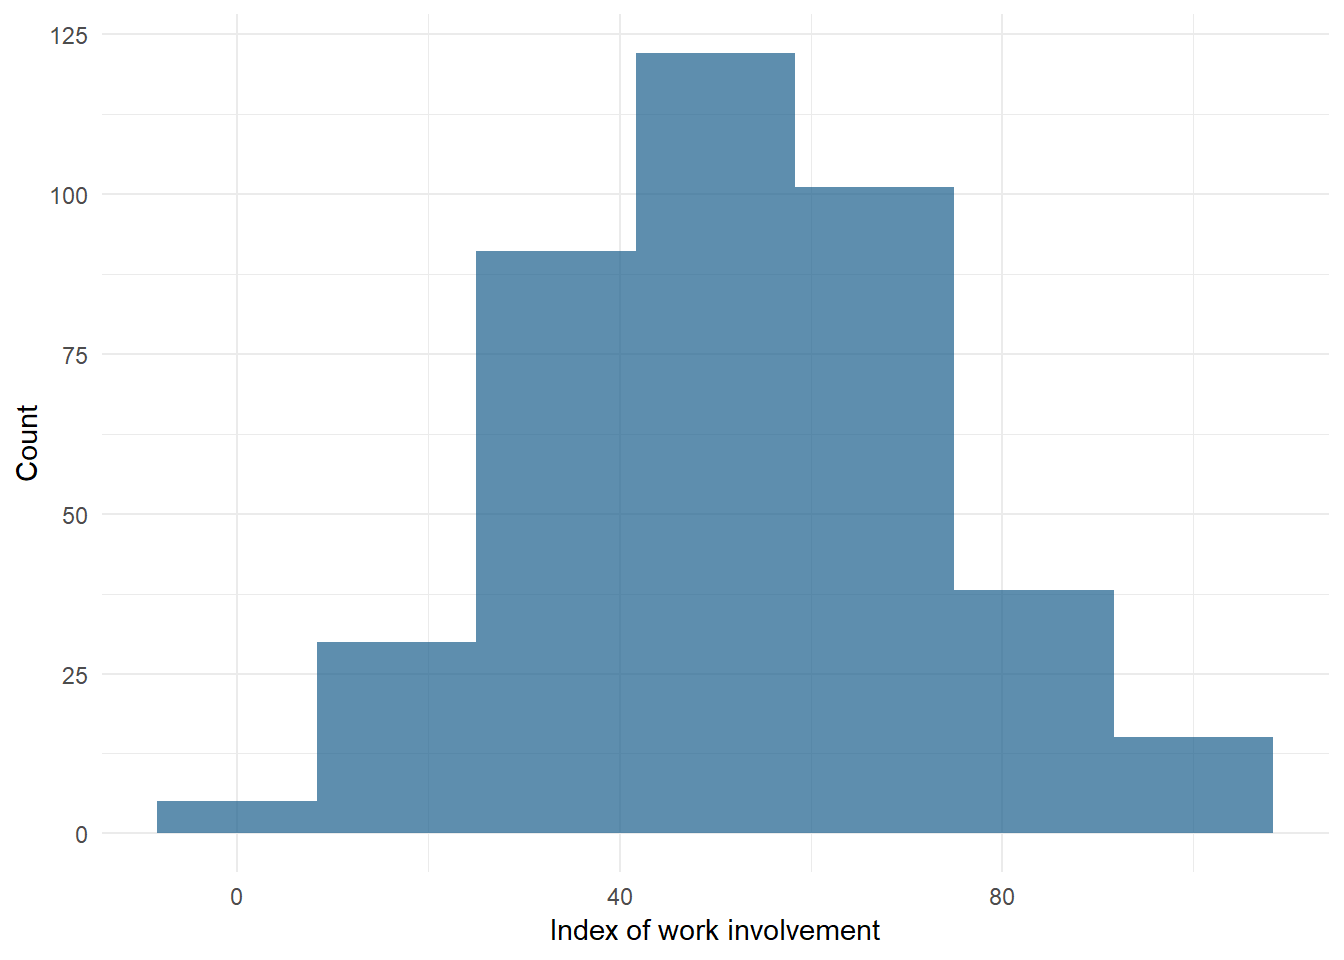
\includegraphics{regression_1_files/figure-latex/unnamed-chunk-13-1} 

}

\caption{Figure 6. Histogram: Index of Work Involvement}\label{fig:unnamed-chunk-13}
\end{figure}

\hypertarget{check-the-relationship-between-variables}{%
\subsubsection{Check the relationship between
variables}\label{check-the-relationship-between-variables}}

I'll now generate scatterplots for DV and all numerical IVs. I will use
partial transparency to indicate strength of the relation in case of the
overlapping data points. Locally estimated scatterplot smoothing (LOESS)
regression lines (Cleveland, 1979; Wickham, 2016) will be added on top
of each scatterplot.

\begin{Shaded}
\begin{Highlighting}[]
\KeywordTok{ggplot}\NormalTok{(data_clean, }\KeywordTok{aes}\NormalTok{(FWI, MONEY)) }\OperatorTok{+}\StringTok{ }\KeywordTok{geom_point}\NormalTok{(}\DataTypeTok{color =}\NormalTok{ color, }
                                          \DataTypeTok{alpha =} \FloatTok{.2}\NormalTok{) }\OperatorTok{+}\StringTok{ }
\StringTok{                               }\KeywordTok{xlab}\NormalTok{(}\StringTok{'Family Wealth Index'}\NormalTok{) }\OperatorTok{+}\StringTok{ }
\StringTok{                               }\KeywordTok{ylab}\NormalTok{(}\StringTok{'Wage'}\NormalTok{) }\OperatorTok{+}\StringTok{ }
\StringTok{                               }\KeywordTok{geom_smooth}\NormalTok{(}\DataTypeTok{color  =}\NormalTok{ color2, }
                                           \DataTypeTok{method =}\StringTok{'loess'}\NormalTok{) }\OperatorTok{+}\StringTok{ }
\StringTok{                               }\KeywordTok{theme_minimal}\NormalTok{()}
\end{Highlighting}
\end{Shaded}

\begin{figure}

{\centering 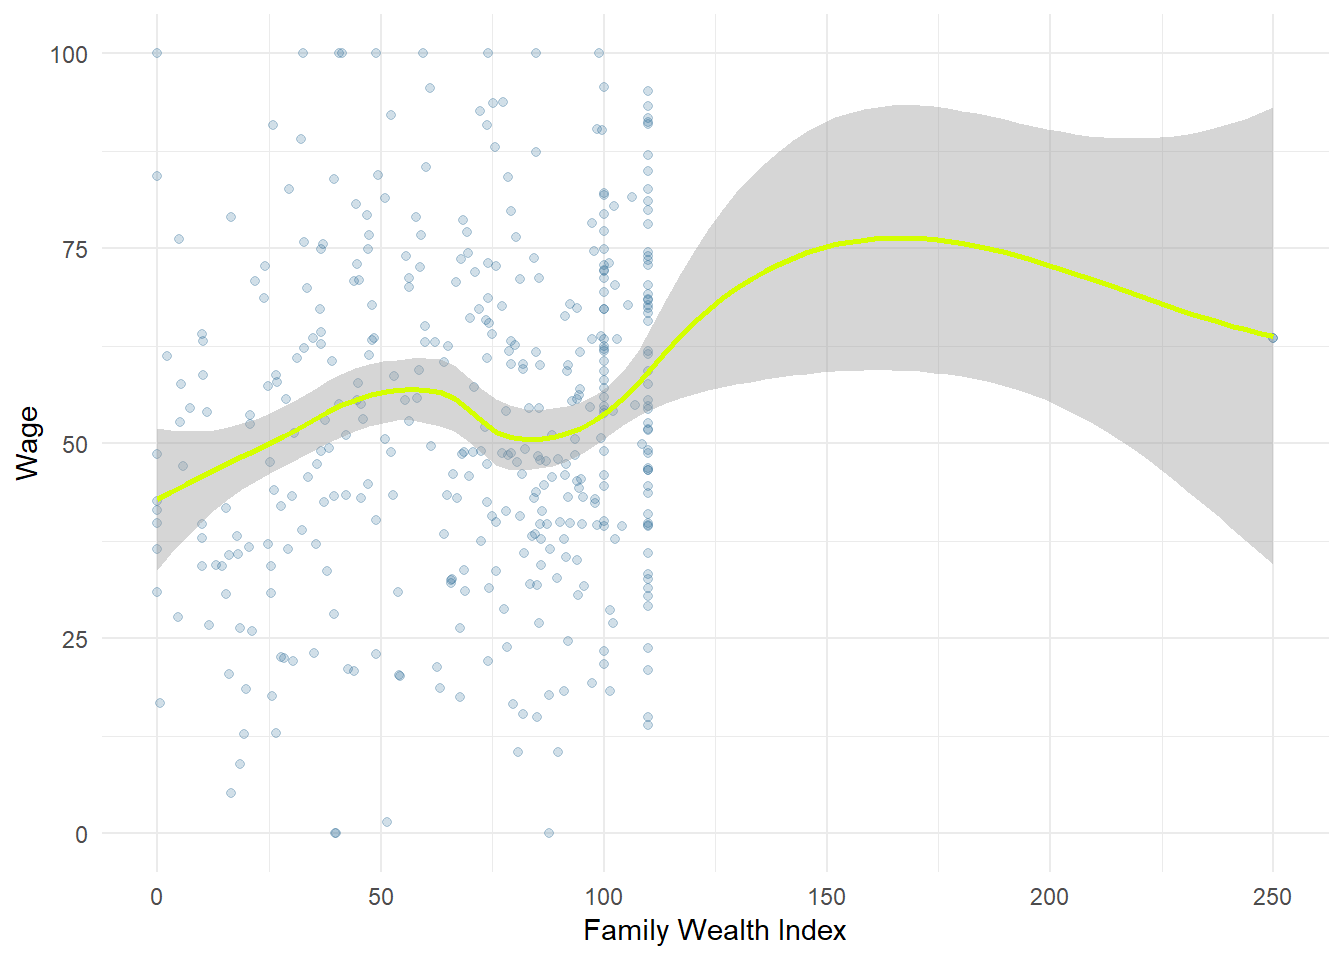
\includegraphics{regression_1_files/figure-latex/unnamed-chunk-14-1} 

}

\caption{Figure 7. Relationship between Wage and Family Wealth Index with added LOESS regression line.}\label{fig:unnamed-chunk-14}
\end{figure}

It seems that the observation taking the value of \texttt{250} is a
serious outlier. Let's make sure if this in an issue with only one data
point.

\begin{Shaded}
\begin{Highlighting}[]
\NormalTok{data_clean}\OperatorTok{$}\NormalTok{FWI[data_clean}\OperatorTok{$}\NormalTok{FWI }\OperatorTok{>}\StringTok{ }\DecValTok{100}\NormalTok{]}
\end{Highlighting}
\end{Shaded}

\begin{verbatim}
##  [1] 101.41 102.11 102.12 102.60 104.19 106.93 108.62 110.00 110.00 110.00
## [11] 110.00 110.00 110.00 110.00 110.00 110.00 110.00 110.00 110.00 110.00
## [21] 110.00 110.00 110.00 110.00 110.00 110.00 110.00 110.00 110.00 110.00
## [31] 110.00 110.00 110.00 110.00 110.00 110.00 110.00 110.00 110.00 110.00
## [41] 250.00 101.13 102.36 102.92 105.47 109.84 110.00 110.00 110.00 110.00
## [51] 110.00 110.00 110.00 110.00 110.00 110.00 110.00 110.00 110.00 110.00
## [61] 110.00 110.00 110.00 110.00 110.00 102.44 110.00 101.49 106.25 250.00
\end{verbatim}

\begin{Shaded}
\begin{Highlighting}[]
\KeywordTok{length}\NormalTok{(data_clean}\OperatorTok{$}\NormalTok{FWI[data_clean}\OperatorTok{$}\NormalTok{FWI }\OperatorTok{>}\StringTok{ }\DecValTok{100}\NormalTok{])}
\end{Highlighting}
\end{Shaded}

\begin{verbatim}
## [1] 70
\end{verbatim}

There are 70 observations with values \texttt{\textgreater{}\ 100}. It
seems reasonable to assume that for \texttt{FWI} the maximum value is
\texttt{110}.

Let's see how many observations take values
\texttt{\textgreater{}\ 110}:

\begin{Shaded}
\begin{Highlighting}[]
\KeywordTok{length}\NormalTok{(data_clean}\OperatorTok{$}\NormalTok{FWI[data_clean}\OperatorTok{$}\NormalTok{FWI }\OperatorTok{>}\StringTok{ }\DecValTok{110}\NormalTok{])}
\end{Highlighting}
\end{Shaded}

\begin{verbatim}
## [1] 2
\end{verbatim}

There are two observations like this. Let's look at them closely:

\begin{Shaded}
\begin{Highlighting}[]
\NormalTok{data_clean}\OperatorTok{$}\NormalTok{FWI[data_clean}\OperatorTok{$}\NormalTok{FWI }\OperatorTok{>}\StringTok{ }\DecValTok{110}\NormalTok{]}
\end{Highlighting}
\end{Shaded}

\begin{verbatim}
## [1] 250 250
\end{verbatim}

Both of them take value of \texttt{250}.

\begin{Shaded}
\begin{Highlighting}[]
\ControlFlowTok{for}\NormalTok{ (col }\ControlFlowTok{in} \KeywordTok{colnames}\NormalTok{(data_clean)) \{}
  \KeywordTok{cat}\NormalTok{(}\StringTok{'Variable'}\NormalTok{, col, }\StringTok{'values for all records with FWI > 110:}\CharTok{\textbackslash{}n}\StringTok{'}\NormalTok{, }\DataTypeTok{sep =} \StringTok{' '}\NormalTok{)}
  \KeywordTok{cat}\NormalTok{(}\KeywordTok{unlist}\NormalTok{(data_clean }\OperatorTok\StringTok{ }\KeywordTok{filter}\NormalTok{(FWI }\OperatorTok{>}\StringTok{ }\DecValTok{110}\NormalTok{) }\OperatorTok\StringTok{ }\KeywordTok{select}\NormalTok{(col)))}
  \KeywordTok{cat}\NormalTok{(}\StringTok{'}\CharTok{\textbackslash{}n\textbackslash{}n}\StringTok{'}\NormalTok{)}
\NormalTok{\}}
\end{Highlighting}
\end{Shaded}

\begin{verbatim}
## Variable MONEY values for all records with FWI > 110:
## 63.55 63.55
## 
## Variable SEX values for all records with FWI > 110:
## 1 1
## 
## Variable FWI values for all records with FWI > 110:
## 250 250
## 
## Variable CI values for all records with FWI > 110:
## 60 60
## 
## Variable AQ values for all records with FWI > 110:
## 93.56 93.56
## 
## Variable II values for all records with FWI > 110:
## 83.51 83.51
## 
## Variable EDUC_elementary values for all records with FWI > 110:
## 1 1
## 
## Variable EDUC_vocational values for all records with FWI > 110:
## 0 0
## 
## Variable EDUC_general_highschool values for all records with FWI > 110:
## 0 0
## 
## Variable EDUC_profiled_highschool values for all records with FWI > 110:
## 0 0
\end{verbatim}

It seems that both cases of \texttt{FWI\ ==\ 250} are in fact the same
observation, but doubled.

We don't know if this value is a result of human coding error or an
artifact generated by some ETL process on the way. As the dataset is big
enough to do so, I decide to delete both observation with
\texttt{FWI\ \textgreater{}\ 110}.

\begin{Shaded}
\begin{Highlighting}[]
\CommentTok{# Remove obs with `FWI` > 110}
\NormalTok{data_clean <-}\StringTok{ }\NormalTok{data_clean }\OperatorTok\StringTok{ }\KeywordTok{filter}\NormalTok{(FWI }\OperatorTok{<=}\StringTok{ }\DecValTok{110}\NormalTok{)}
\end{Highlighting}
\end{Shaded}

\begin{Shaded}
\begin{Highlighting}[]
\CommentTok{# Sanity check}
\KeywordTok{sum}\NormalTok{(data_clean}\OperatorTok{$}\NormalTok{FWI }\OperatorTok{>}\StringTok{ }\DecValTok{110}\NormalTok{)}
\end{Highlighting}
\end{Shaded}

\begin{verbatim}
## [1] 0
\end{verbatim}

Another potential problem in the \texttt{FWI} is it's max value. From
the scatterplot it seems that there's a bounding value of \texttt{100}
and then another one at \texttt{110}. This is a possible indicator of
measurement error. Another explanation could be that, there's a ceiling
effect for some groups or sub-groups.

Note that variance of \texttt{FWI} seems to be smaller between
\texttt{100} and \texttt{110} than in the range of 0 - 100. This might
be problematic in the context of homo-/heteroscedasticity. I'll keep
that in mind and move forward. We'll come back to these issues when
diagnosing the model.

Now let's get back to scatter plots.

\begin{Shaded}
\begin{Highlighting}[]
\KeywordTok{ggplot}\NormalTok{(data_clean, }\KeywordTok{aes}\NormalTok{(FWI, MONEY)) }\OperatorTok{+}\StringTok{ }\KeywordTok{geom_point}\NormalTok{(}\DataTypeTok{color =}\NormalTok{ color, }
                                          \DataTypeTok{alpha =} \FloatTok{.2}\NormalTok{) }\OperatorTok{+}\StringTok{ }
\StringTok{                               }\KeywordTok{xlab}\NormalTok{(}\StringTok{'Family Wealth Index'}\NormalTok{) }\OperatorTok{+}\StringTok{ }
\StringTok{                               }\KeywordTok{ylab}\NormalTok{(}\StringTok{'Wage'}\NormalTok{) }\OperatorTok{+}\StringTok{ }
\StringTok{                               }\KeywordTok{geom_smooth}\NormalTok{(}\DataTypeTok{color  =}\NormalTok{ color2, }
                                           \DataTypeTok{method =}\StringTok{'loess'}\NormalTok{) }\OperatorTok{+}\StringTok{ }
\StringTok{                               }\KeywordTok{theme_minimal}\NormalTok{()}
\end{Highlighting}
\end{Shaded}

\begin{figure}

{\centering 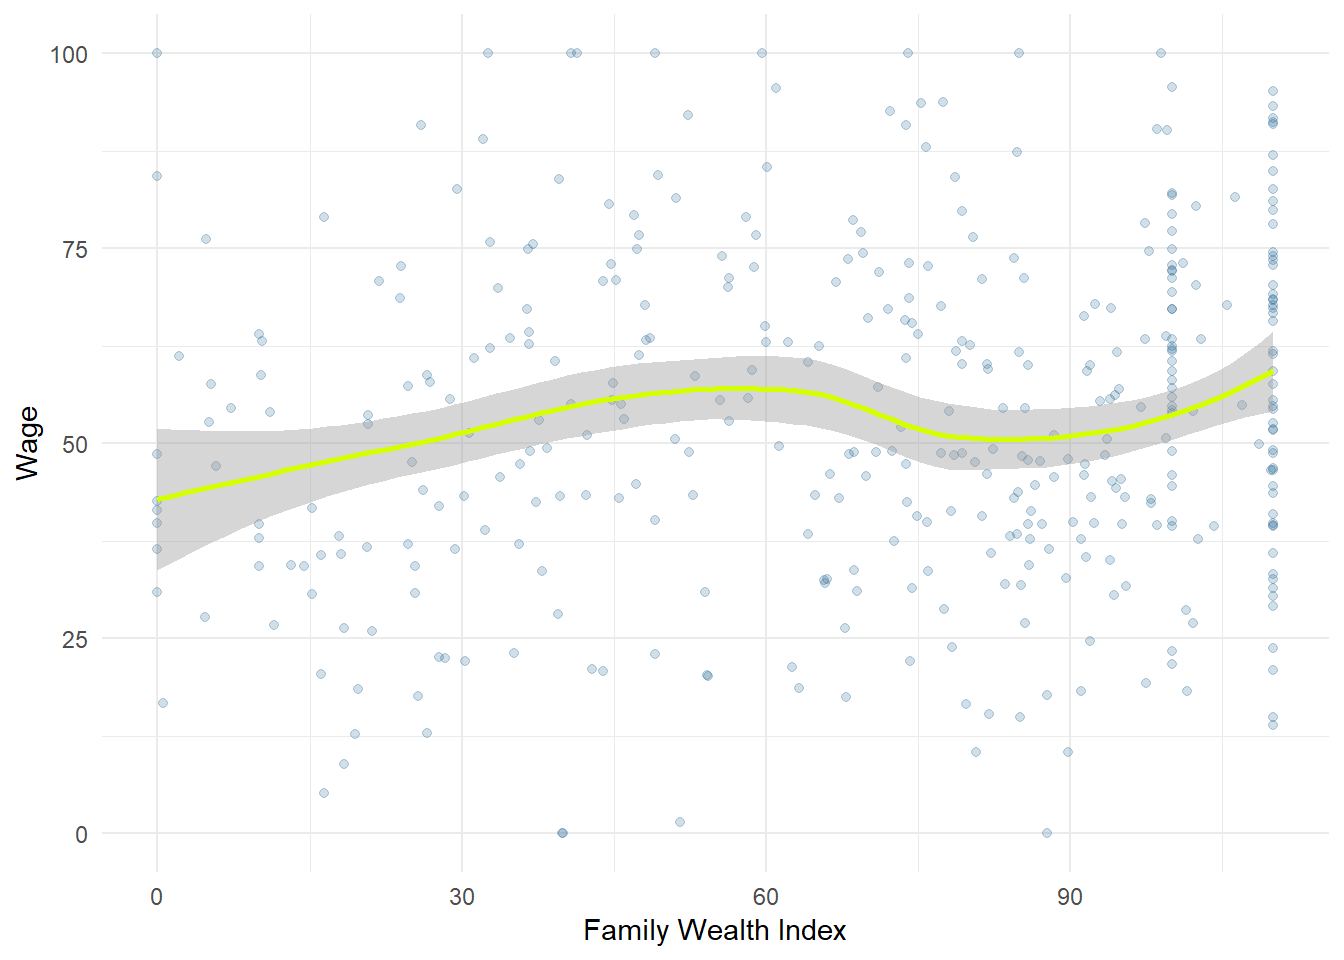
\includegraphics{regression_1_files/figure-latex/unnamed-chunk-22-1} 

}

\caption{Figure 8. Relationship between Wage and Family Wealth Index with added LOESS regression line (outliers removed).}\label{fig:unnamed-chunk-22}
\end{figure}

\begin{Shaded}
\begin{Highlighting}[]
\KeywordTok{ggplot}\NormalTok{(data_clean, }\KeywordTok{aes}\NormalTok{(CI, MONEY)) }\OperatorTok{+}\StringTok{ }\KeywordTok{geom_point}\NormalTok{(}\DataTypeTok{color =}\NormalTok{ color, }
                                          \DataTypeTok{alpha =} \FloatTok{.2}\NormalTok{) }\OperatorTok{+}\StringTok{ }
\StringTok{                               }\KeywordTok{xlab}\NormalTok{(}\StringTok{'Competence Assesment Index'}\NormalTok{) }\OperatorTok{+}\StringTok{ }
\StringTok{                               }\KeywordTok{ylab}\NormalTok{(}\StringTok{'Wage'}\NormalTok{) }\OperatorTok{+}\StringTok{ }
\StringTok{                               }\KeywordTok{geom_smooth}\NormalTok{(}\DataTypeTok{color  =}\NormalTok{ color2, }
                                           \DataTypeTok{method =}\StringTok{'loess'}\NormalTok{) }\OperatorTok{+}\StringTok{ }
\StringTok{                               }\KeywordTok{theme_minimal}\NormalTok{()}
\end{Highlighting}
\end{Shaded}

\begin{figure}

{\centering 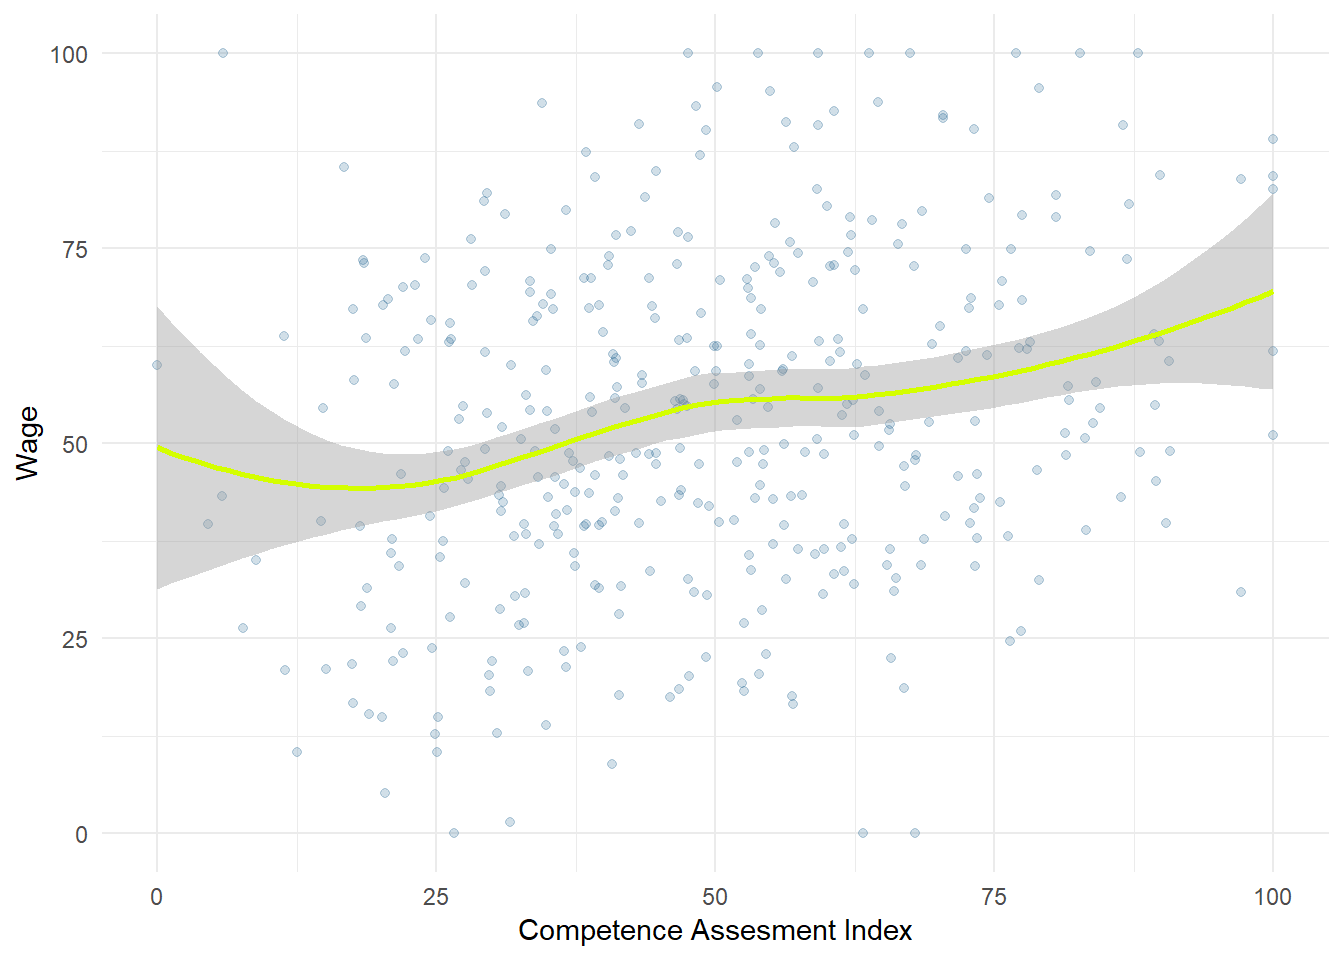
\includegraphics{regression_1_files/figure-latex/unnamed-chunk-23-1} 

}

\caption{Figure 9. Relationship between Wage and Competence Assesment Index with added LOESS regression line.}\label{fig:unnamed-chunk-23}
\end{figure}

\begin{Shaded}
\begin{Highlighting}[]
\KeywordTok{ggplot}\NormalTok{(data_clean, }\KeywordTok{aes}\NormalTok{(AQ, MONEY)) }\OperatorTok{+}\StringTok{ }\KeywordTok{geom_point}\NormalTok{(}\DataTypeTok{color =}\NormalTok{ color, }
                                          \DataTypeTok{alpha =} \FloatTok{.2}\NormalTok{) }\OperatorTok{+}\StringTok{ }
\StringTok{                               }\KeywordTok{xlab}\NormalTok{(}\StringTok{'Ambitions Questionnaire Index'}\NormalTok{) }\OperatorTok{+}\StringTok{ }
\StringTok{                               }\KeywordTok{ylab}\NormalTok{(}\StringTok{'Wage'}\NormalTok{) }\OperatorTok{+}\StringTok{ }
\StringTok{                               }\KeywordTok{geom_smooth}\NormalTok{(}\DataTypeTok{color  =}\NormalTok{ color2, }
                                           \DataTypeTok{method =}\StringTok{'loess'}\NormalTok{) }\OperatorTok{+}\StringTok{ }
\StringTok{                               }\KeywordTok{theme_minimal}\NormalTok{()}
\end{Highlighting}
\end{Shaded}

\begin{figure}

{\centering 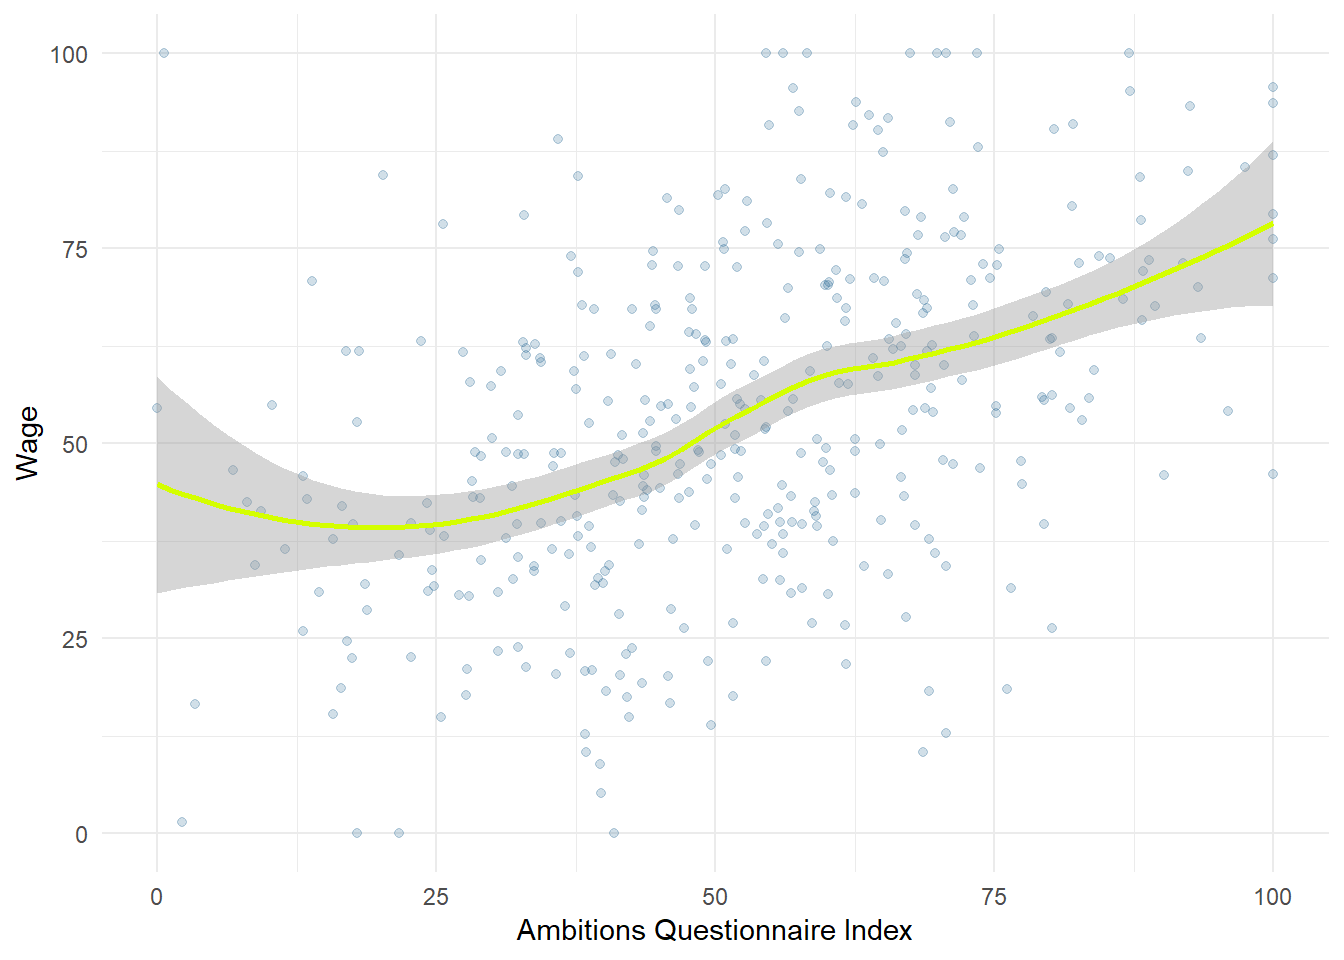
\includegraphics{regression_1_files/figure-latex/unnamed-chunk-24-1} 

}

\caption{Figure 10. Relationship between Wage and Ambitions Questionnaire Index with added LOESS regression line.}\label{fig:unnamed-chunk-24}
\end{figure}

\begin{Shaded}
\begin{Highlighting}[]
\KeywordTok{ggplot}\NormalTok{(data_clean, }\KeywordTok{aes}\NormalTok{(II, MONEY)) }\OperatorTok{+}\StringTok{ }\KeywordTok{geom_point}\NormalTok{(}\DataTypeTok{color =}\NormalTok{ color, }
                                          \DataTypeTok{alpha =} \FloatTok{.2}\NormalTok{) }\OperatorTok{+}\StringTok{ }
\StringTok{                               }\KeywordTok{xlab}\NormalTok{(}\StringTok{'Index of Work Involvement'}\NormalTok{) }\OperatorTok{+}\StringTok{ }
\StringTok{                               }\KeywordTok{ylab}\NormalTok{(}\StringTok{'Wage'}\NormalTok{) }\OperatorTok{+}\StringTok{ }
\StringTok{                               }\KeywordTok{geom_smooth}\NormalTok{(}\DataTypeTok{color  =}\NormalTok{ color2, }
                                           \DataTypeTok{method =}\StringTok{'loess'}\NormalTok{) }\OperatorTok{+}\StringTok{ }
\StringTok{                               }\KeywordTok{theme_minimal}\NormalTok{()}
\end{Highlighting}
\end{Shaded}

\begin{figure}

{\centering 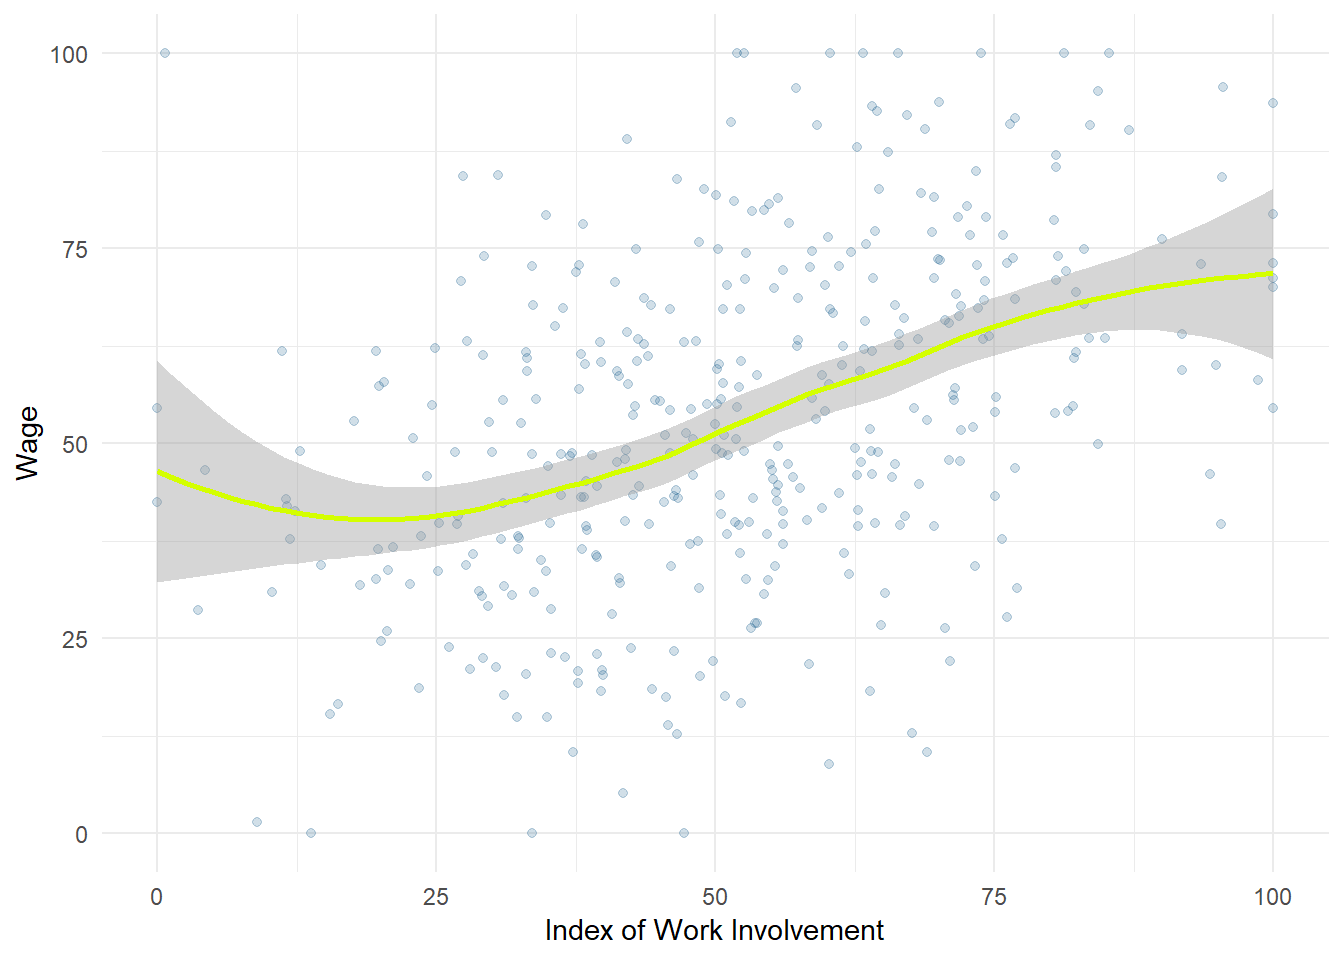
\includegraphics{regression_1_files/figure-latex/unnamed-chunk-25-1} 

}

\caption{Figure 11. Relationship between Wage and Index of Work Involvement with added LOESS regression line.}\label{fig:unnamed-chunk-25}
\end{figure}

\hypertarget{assumptions-of-linear-regression}{%
\subsection{Assumptions of linear
regression}\label{assumptions-of-linear-regression}}

\hypertarget{linearity}{%
\subsubsection{Linearity}\label{linearity}}

From the scatterplots above we can see that most of the variables have
reasonably linear relationship with DV. Again, \texttt{FWI} is the most
controversial in this regard. Let's run full diagnostics to check if and
to what extent it's problematic.

To run diagnostics we need to fit the model first.

\begin{Shaded}
\begin{Highlighting}[]
\NormalTok{model_}\DecValTok{1}\NormalTok{ <-}\StringTok{ }\KeywordTok{lm}\NormalTok{(MONEY }\OperatorTok{~}\StringTok{ }\NormalTok{., }\DataTypeTok{data =}\NormalTok{ data_clean)}
\end{Highlighting}
\end{Shaded}

Let's see model summary.

\begin{Shaded}
\begin{Highlighting}[]
\KeywordTok{summary}\NormalTok{(model_}\DecValTok{1}\NormalTok{)}
\end{Highlighting}
\end{Shaded}

\begin{verbatim}
## 
## Call:
## lm(formula = MONEY ~ ., data = data_clean)
## 
## Residuals:
##     Min      1Q  Median      3Q     Max 
## -46.687 -10.426   0.527   9.072 121.373 
## 
## Coefficients:
##                           Estimate Std. Error t value Pr(>|t|)    
## (Intercept)               -8.95837    4.07671  -2.197  0.02858 *  
## SEX                       -5.82127    1.79324  -3.246  0.00127 ** 
## FWI                        0.39368    0.04741   8.303 1.69e-15 ***
## CI                         0.53242    0.04119  12.925  < 2e-16 ***
## AQ                         0.26817    0.08384   3.199  0.00149 ** 
## II                         0.24043    0.08515   2.823  0.00499 ** 
## EDUC_elementary          -29.64181    3.82881  -7.742 8.52e-14 ***
## EDUC_vocational          -22.44630    3.37066  -6.659 9.37e-11 ***
## EDUC_general_highschool   -8.98810    3.03276  -2.964  0.00323 ** 
## EDUC_profiled_highschool -10.05573    2.96285  -3.394  0.00076 ***
## ---
## Signif. codes:  0 '***' 0.001 '**' 0.01 '*' 0.05 '.' 0.1 ' ' 1
## 
## Residual standard error: 15.47 on 390 degrees of freedom
## Multiple R-squared:  0.4885, Adjusted R-squared:  0.4767 
## F-statistic: 41.39 on 9 and 390 DF,  p-value: < 2.2e-16
\end{verbatim}

According to repective \(t\) and \(p\) values all the variables are
significant predictors of the outcome variable. As indicated by the
\(F\) test (\(F(9, 390) = 41.39, p < .001\)) \texttt{model\_1} provides
a better fit to the data than a model that contains no independent
variables. It remains an open question if dummy recoded \texttt{EDUC} as
a whole is a significant predictor of \(DV\). We'll test for this later.

\hypertarget{outliers-and-influential-cases}{%
\subsubsection{Outliers and influential
cases}\label{outliers-and-influential-cases}}

\begin{Shaded}
\begin{Highlighting}[]
\KeywordTok{autoplot}\NormalTok{(model_}\DecValTok{1}\NormalTok{, }\DataTypeTok{colour =}\NormalTok{ color, }\DataTypeTok{smooth.colour =}\NormalTok{ color3, }\DataTypeTok{alpha =} \FloatTok{.3}\NormalTok{) }\OperatorTok{+}\StringTok{ }\KeywordTok{theme_minimal}\NormalTok{()}
\end{Highlighting}
\end{Shaded}

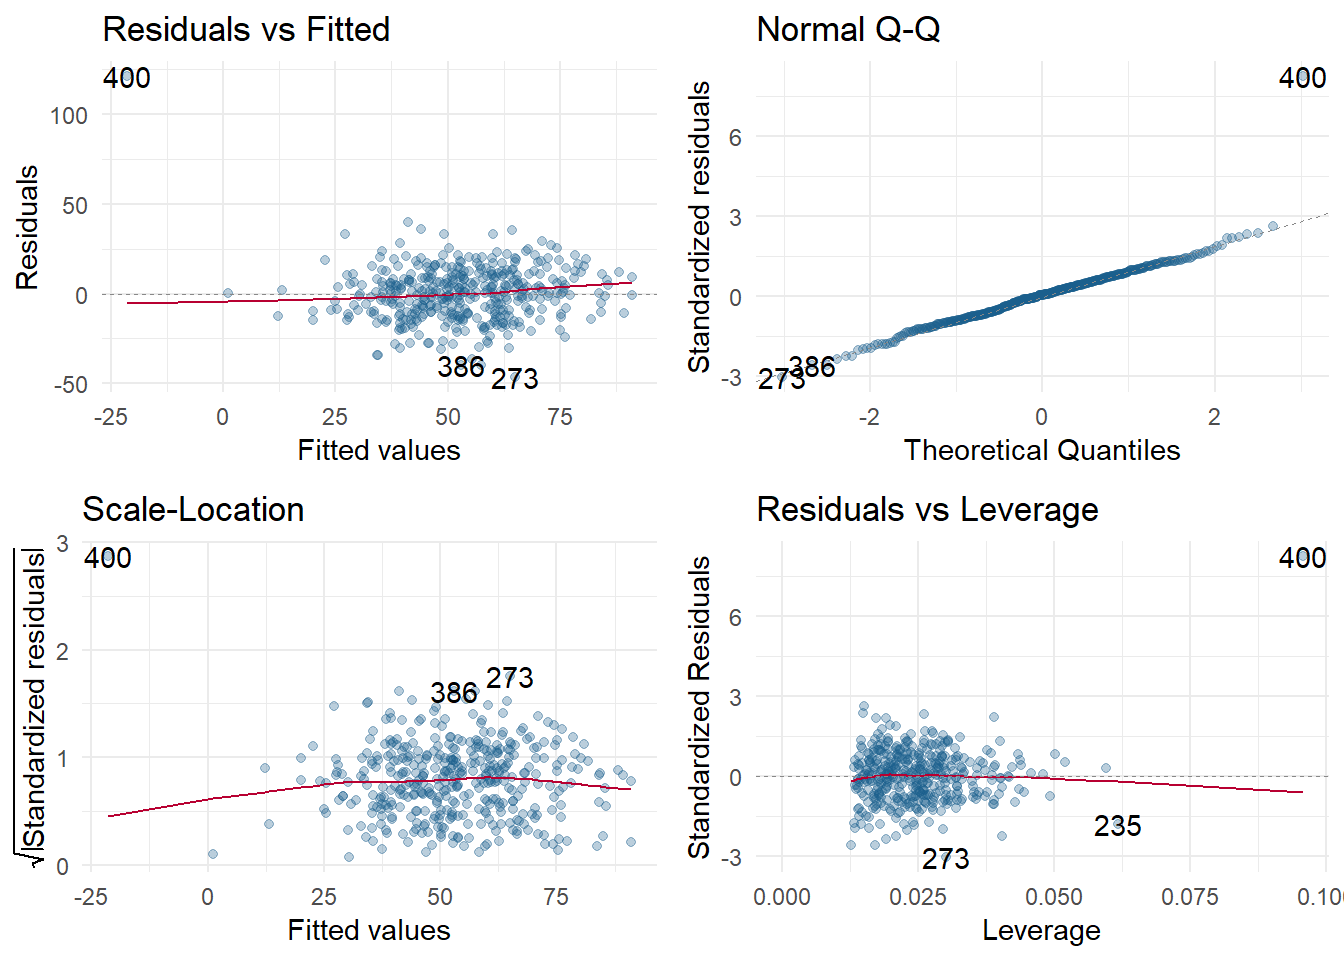
\includegraphics{regression_1_files/figure-latex/unnamed-chunk-28-1.pdf}

It seems that observation number \texttt{400} is highly problematic.
Let's assess its impact on the model.

\begin{Shaded}
\begin{Highlighting}[]
\CommentTok{# Standardized DFBETAS}
\NormalTok{dfb_model_}\DecValTok{1}\NormalTok{ <-}\StringTok{ }\KeywordTok{dfbetas}\NormalTok{(model_}\DecValTok{1}\NormalTok{)}
\KeywordTok{sum}\NormalTok{(}\KeywordTok{abs}\NormalTok{(dfb_model_}\DecValTok{1}\NormalTok{) }\OperatorTok{>}\StringTok{ }\NormalTok{(}\DecValTok{2} \OperatorTok{/}\StringTok{ }\KeywordTok{sqrt}\NormalTok{(}\KeywordTok{dim}\NormalTok{(data_clean)[}\DecValTok{1}\NormalTok{])))}
\end{Highlighting}
\end{Shaded}

\begin{verbatim}
## [1] 193
\end{verbatim}

According to a heuristic strategy (\(|DFBETA| > \frac{2}{\sqrt{N}}\))
there are \(193\) outlying observations. It does not seem reasonable
after examining diagnostic plot. Let's see other metrics.

\begin{Shaded}
\begin{Highlighting}[]
\CommentTok{# Standardize DFFITS}
\NormalTok{dffits_vec <-}\StringTok{ }\KeywordTok{dffits}\NormalTok{(model_}\DecValTok{1}\NormalTok{) }\OperatorTok{>}\StringTok{ }\NormalTok{(}\DecValTok{2} \OperatorTok{/}\StringTok{ }\KeywordTok{sqrt}\NormalTok{(}\KeywordTok{dim}\NormalTok{(data_clean)[}\DecValTok{2}\NormalTok{] }\OperatorTok{/}\StringTok{ }\KeywordTok{dim}\NormalTok{(data_clean[}\DecValTok{1}\NormalTok{])))}
\KeywordTok{cat}\NormalTok{(}\KeywordTok{which}\NormalTok{(dffits_vec }\OperatorTok{==}\StringTok{ }\OtherTok{TRUE}\NormalTok{))}
\end{Highlighting}
\end{Shaded}

\begin{verbatim}
## 400
\end{verbatim}

DFFITS point to one problematic observation - observation \texttt{400}.

\begin{Shaded}
\begin{Highlighting}[]
\CommentTok{# Leverage statistic}
\NormalTok{hatvals <-}\StringTok{ }\KeywordTok{hatvalues}\NormalTok{(model_}\DecValTok{1}\NormalTok{)}
\KeywordTok{cat}\NormalTok{(}\StringTok{'More conservative criterion:'}\NormalTok{)}
\end{Highlighting}
\end{Shaded}

\begin{verbatim}
## More conservative criterion:
\end{verbatim}

\begin{Shaded}
\begin{Highlighting}[]
\KeywordTok{cat}\NormalTok{(}\KeywordTok{which}\NormalTok{((hatvals }\OperatorTok{>}\StringTok{ }\DecValTok{2}\OperatorTok{*}\NormalTok{(}\KeywordTok{dim}\NormalTok{(data_clean)[}\DecValTok{2}\NormalTok{] }\OperatorTok{/}\StringTok{ }\KeywordTok{dim}\NormalTok{(data_clean)[}\DecValTok{1}\NormalTok{])) }\OperatorTok{==}\StringTok{ }\OtherTok{TRUE}\NormalTok{))}
\end{Highlighting}
\end{Shaded}

\begin{verbatim}
## 224 234 235 246 400
\end{verbatim}

\begin{Shaded}
\begin{Highlighting}[]
\KeywordTok{cat}\NormalTok{(}\StringTok{'Less conservative criterion:'}\NormalTok{)}
\end{Highlighting}
\end{Shaded}

\begin{verbatim}
## Less conservative criterion:
\end{verbatim}

\begin{Shaded}
\begin{Highlighting}[]
\KeywordTok{cat}\NormalTok{(}\KeywordTok{which}\NormalTok{((hatvals }\OperatorTok{>}\StringTok{ }\DecValTok{3}\OperatorTok{*}\NormalTok{(}\KeywordTok{dim}\NormalTok{(data_clean)[}\DecValTok{2}\NormalTok{] }\OperatorTok{/}\StringTok{ }\KeywordTok{dim}\NormalTok{(data_clean)[}\DecValTok{1}\NormalTok{])) }\OperatorTok{==}\StringTok{ }\OtherTok{TRUE}\NormalTok{))}
\end{Highlighting}
\end{Shaded}

\begin{verbatim}
## 400
\end{verbatim}

Leverage statistic points to observations \texttt{224}, \texttt{234},
\texttt{235}, \texttt{246}, and \texttt{400} (more conservative) or only
\texttt{400} (less conservative) as problematic (Sarkar, nd)

\begin{Shaded}
\begin{Highlighting}[]
\CommentTok{# Cook's distance}
\NormalTok{c_dist <-}\StringTok{ }\KeywordTok{cooks.distance}\NormalTok{(model_}\DecValTok{1}\NormalTok{)}
\KeywordTok{sum}\NormalTok{(c_dist }\OperatorTok{>}\StringTok{ }\DecValTok{1}\NormalTok{)}
\end{Highlighting}
\end{Shaded}

\begin{verbatim}
## [1] 0
\end{verbatim}

As suggested by Cook (1982), observations with \(D_i > 1\) can be
interpreted as influential when the dataset is `large enough' (Cook et
al., 1982). There are no such observations in the data.

Another heuristic says that observations with \(D_i > 3 * \mu(D)\) can
be treated as influential.

\begin{Shaded}
\begin{Highlighting}[]
\KeywordTok{which}\NormalTok{((c_dist }\OperatorTok{>}\StringTok{ }\DecValTok{3}\OperatorTok{*}\KeywordTok{mean}\NormalTok{(c_dist)) }\OperatorTok{==}\StringTok{ }\OtherTok{TRUE}\NormalTok{)}
\end{Highlighting}
\end{Shaded}

\begin{verbatim}
##  83 101 235 241 273 309 386 400 
##  83 101 235 241 273 309 386 400
\end{verbatim}

This heuristic reveals that following obseravtions might cause problems:

\texttt{83}, \texttt{101}, \texttt{235}, \texttt{241}, \texttt{273},
\texttt{309}, \texttt{386}, \texttt{400}.

Observation \texttt{400} seems the most problematic.

It also seems very extreme and unlikely to bring any business value.

I decide to remove this observation and re-fit the model.

\begin{Shaded}
\begin{Highlighting}[]
\NormalTok{data_clean_NO <-}\StringTok{ }\NormalTok{data_clean }\OperatorTok\StringTok{ }\KeywordTok{slice}\NormalTok{(}\OperatorTok{-}\DecValTok{400}\NormalTok{)}
\end{Highlighting}
\end{Shaded}

Re-fit the model.

\begin{Shaded}
\begin{Highlighting}[]
\NormalTok{model_}\DecValTok{2}\NormalTok{ <-}\StringTok{ }\KeywordTok{lm}\NormalTok{(MONEY }\OperatorTok{~}\StringTok{ }\NormalTok{., data_clean_NO)}
\end{Highlighting}
\end{Shaded}

\begin{Shaded}
\begin{Highlighting}[]
\KeywordTok{summary}\NormalTok{(model_}\DecValTok{2}\NormalTok{)}
\end{Highlighting}
\end{Shaded}

\begin{verbatim}
## 
## Call:
## lm(formula = MONEY ~ ., data = data_clean_NO)
## 
## Residuals:
##     Min      1Q  Median      3Q     Max 
## -45.447  -9.528   0.358   9.589  41.285 
## 
## Coefficients:
##                           Estimate Std. Error t value Pr(>|t|)    
## (Intercept)              -16.00501    3.78899  -4.224 2.99e-05 ***
## SEX                       -7.82985    1.64624  -4.756 2.78e-06 ***
## FWI                        0.46647    0.04387  10.633  < 2e-16 ***
## CI                         0.59540    0.03811  15.623  < 2e-16 ***
## AQ                         0.27071    0.07627   3.549 0.000433 ***
## II                         0.28051    0.07759   3.615 0.000339 ***
## EDUC_elementary          -33.94305    3.51512  -9.656  < 2e-16 ***
## EDUC_vocational          -25.96466    3.09065  -8.401 8.40e-16 ***
## EDUC_general_highschool  -10.80376    2.76609  -3.906 0.000111 ***
## EDUC_profiled_highschool -14.24437    2.73452  -5.209 3.08e-07 ***
## ---
## Signif. codes:  0 '***' 0.001 '**' 0.01 '*' 0.05 '.' 0.1 ' ' 1
## 
## Residual standard error: 14.07 on 389 degrees of freedom
## Multiple R-squared:  0.5727, Adjusted R-squared:  0.5628 
## F-statistic: 57.92 on 9 and 389 DF,  p-value: < 2.2e-16
\end{verbatim}

The fit seems much better as expressed by lower \(p\) and higher \(R^2\)
(\(R^2_{adj} = .48\) vs \(R^2_{adj} = .56\)) values. The new model
offers better fit to the data than model with no predictors as indicated
by \(F\) test (\(F(9, 389) = 57.92, p < .001\))

Let's examine diagnostic plots of the new fit:

\begin{Shaded}
\begin{Highlighting}[]
\KeywordTok{autoplot}\NormalTok{(model_}\DecValTok{2}\NormalTok{, }\DataTypeTok{colour =}\NormalTok{ color, }\DataTypeTok{smooth.colour =}\NormalTok{ color3, }\DataTypeTok{alpha =} \FloatTok{.3}\NormalTok{) }\OperatorTok{+}\StringTok{ }\KeywordTok{theme_minimal}\NormalTok{()}
\end{Highlighting}
\end{Shaded}

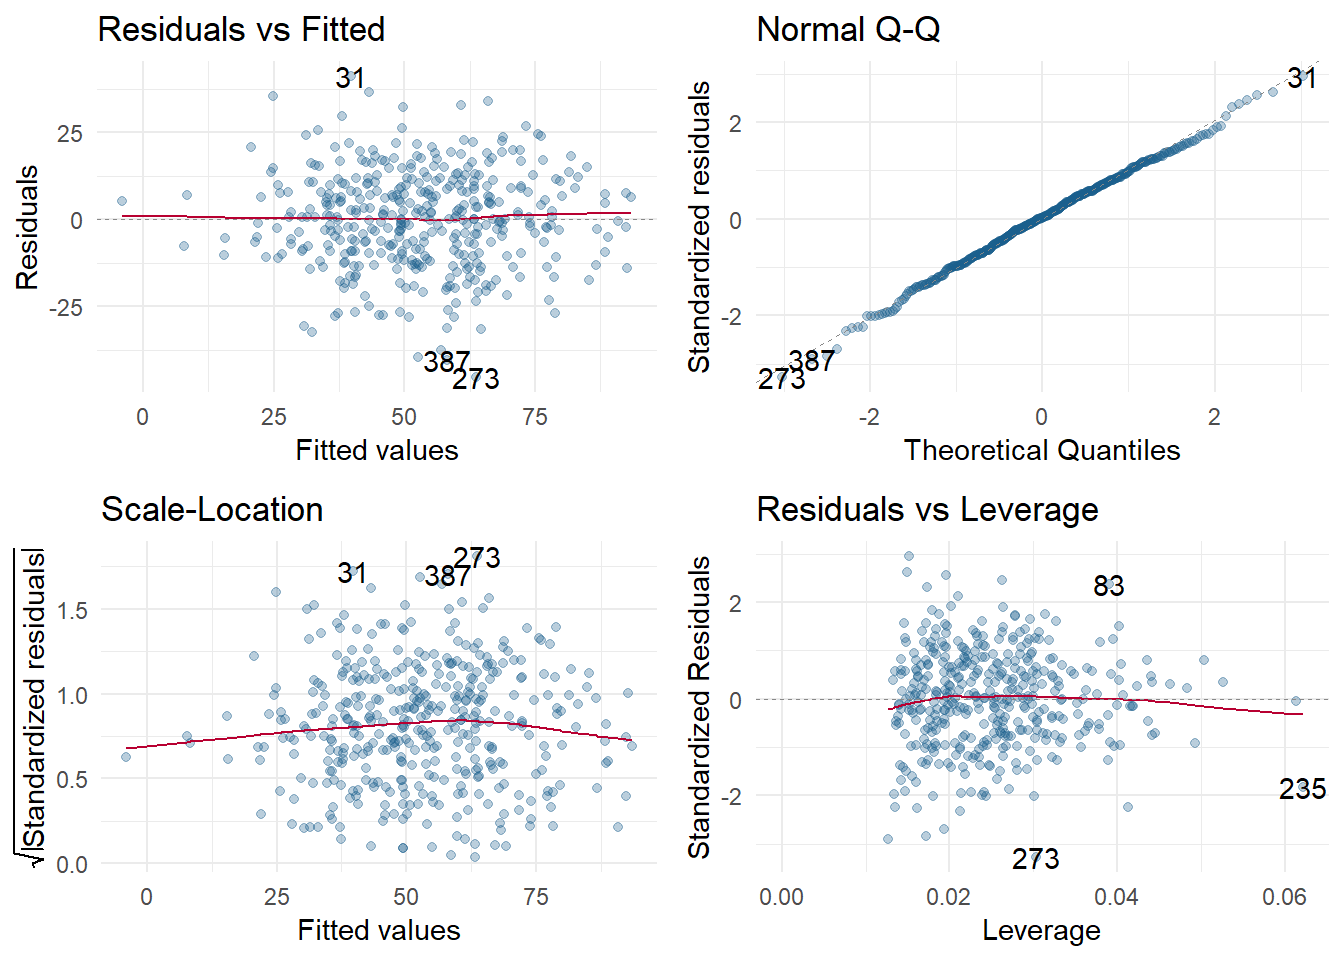
\includegraphics{regression_1_files/figure-latex/unnamed-chunk-37-1.pdf}

The current plots indicate that:

\begin{itemize}
\item
  Linearity assumption is fulfilled (fitted values vs residuals plot)
\item
  Normal Q-Q plot indicates that distribution of residuals is normal or
  very close to normal
\item
  Scale location plot reveals that there might be a slight problem with
  homoscedasticity.
\item
  Residual vs leverage plot indicates that there are no extreme outliers
  / influential cases anymore. Further deletions could possibly improve
  the model fit (e.g.~deletions of points \texttt{235} or \texttt{273}),
  but that could possibly cause overfitting and hurt model's over
  generalizability and predictive power.
\end{itemize}

\hypertarget{homoscedasticity}{%
\subsubsection{Homoscedasticity}\label{homoscedasticity}}

Building on top of visual inspection, let's check heteroscedasticity
using Breush-Pagan and NCV tests.

\begin{Shaded}
\begin{Highlighting}[]
\NormalTok{lmtest}\OperatorTok{::}\KeywordTok{bptest}\NormalTok{(model_}\DecValTok{2}\NormalTok{)}
\end{Highlighting}
\end{Shaded}

\begin{verbatim}
## 
##  studentized Breusch-Pagan test
## 
## data:  model_2
## BP = 5.2944, df = 9, p-value = 0.8079
\end{verbatim}

\begin{Shaded}
\begin{Highlighting}[]
\NormalTok{car}\OperatorTok{::}\KeywordTok{ncvTest}\NormalTok{(model_}\DecValTok{2}\NormalTok{)}
\end{Highlighting}
\end{Shaded}

\begin{verbatim}
## Non-constant Variance Score Test 
## Variance formula: ~ fitted.values 
## Chisquare = 0.02481138, Df = 1, p = 0.87484
\end{verbatim}

Both tests demonstrated insignificant result at customary level
\(p < .05\). We can assume that homoscedasticity assumption is met.

\hypertarget{multicollinearity}{%
\subsubsection{Multicollinearity}\label{multicollinearity}}

Now, let's examine if the model does not suffer from multicollinearity.

\begin{Shaded}
\begin{Highlighting}[]
\CommentTok{# Correlation matrix}
\NormalTok{cor_mtrx <-}\StringTok{ }\KeywordTok{cor}\NormalTok{(data_clean_NO)}
\end{Highlighting}
\end{Shaded}

\begin{Shaded}
\begin{Highlighting}[]
\CommentTok{# Check all corrs > .8}
\KeywordTok{which}\NormalTok{((cor_mtrx[cor_mtrx }\OperatorTok{>}\StringTok{ }\FloatTok{.8}\NormalTok{] }\OperatorTok{&&}\StringTok{ }\NormalTok{cor_mtrx[cor_mtrx }\OperatorTok{!=}\StringTok{ }\DecValTok{1}\NormalTok{]) }\OperatorTok{==}\StringTok{ }\OtherTok{TRUE}\NormalTok{)}
\end{Highlighting}
\end{Shaded}

\begin{verbatim}
## [1] 1
\end{verbatim}

\begin{Shaded}
\begin{Highlighting}[]
\KeywordTok{print}\NormalTok{(}\KeywordTok{cor.test}\NormalTok{(data_clean_NO}\OperatorTok{$}\NormalTok{AQ, data_clean_NO}\OperatorTok{$}\NormalTok{II))}
\end{Highlighting}
\end{Shaded}

\begin{verbatim}
## 
##  Pearson's product-moment correlation
## 
## data:  data_clean_NO$AQ and data_clean_NO$II
## t = 38.626, df = 397, p-value < 2.2e-16
## alternative hypothesis: true correlation is not equal to 0
## 95 percent confidence interval:
##  0.8661220 0.9077041
## sample estimates:
##       cor 
## 0.8887271
\end{verbatim}

It seems that correlation between \texttt{AQ} and \texttt{II} might be
potentially problematic. Let's see Variance Inflation Factor values for
\texttt{model\_2}.

\begin{Shaded}
\begin{Highlighting}[]
\NormalTok{model_}\DecValTok{2}\NormalTok{_vif =}\StringTok{ }\KeywordTok{vif}\NormalTok{(model_}\DecValTok{2}\NormalTok{)}
\KeywordTok{print}\NormalTok{(model_}\DecValTok{2}\NormalTok{_vif)}
\end{Highlighting}
\end{Shaded}

\begin{verbatim}
##                      SEX                      FWI                       CI 
##                 1.365538                 4.015182                 1.217330 
##                       AQ                       II          EDUC_elementary 
##                 4.914089                 4.923837                 4.677225 
##          EDUC_vocational  EDUC_general_highschool EDUC_profiled_highschool 
##                 3.615828                 1.661241                 1.651934
\end{verbatim}

\begin{Shaded}
\begin{Highlighting}[]
\KeywordTok{cat}\NormalTok{(}\StringTok{"}\CharTok{\textbackslash{}n}\StringTok{Tolerance: "}\NormalTok{, }\DecValTok{1} \OperatorTok{/}\StringTok{ }\NormalTok{model_}\DecValTok{2}\NormalTok{_vif)}
\end{Highlighting}
\end{Shaded}

\begin{verbatim}
## 
## Tolerance:  0.7323121 0.2490547 0.8214697 0.2034965 0.2030937 0.213802 0.2765619 0.6019595 0.605351
\end{verbatim}

A well known heuristic says that when \(VIF < 5\) then model does not
suffer a serious multicollinearity.

Nevertheless, let's temporarily remove one of the highest VIF variables
and see how it influences model fit. \(VIF\) is the highest for
\texttt{II}.

\begin{Shaded}
\begin{Highlighting}[]
\NormalTok{model_}\DecValTok{2}\NormalTok{_}\DecValTok{1}\NormalTok{ <-}\StringTok{ }\KeywordTok{lm}\NormalTok{(MONEY }\OperatorTok{~}\StringTok{ }\NormalTok{., data_clean_NO }\OperatorTok\StringTok{ }\KeywordTok{select}\NormalTok{(}\OperatorTok{-}\NormalTok{II))}
\end{Highlighting}
\end{Shaded}

\begin{Shaded}
\begin{Highlighting}[]
\KeywordTok{summary}\NormalTok{(model_}\DecValTok{2}\NormalTok{_}\DecValTok{1}\NormalTok{)}
\end{Highlighting}
\end{Shaded}

\begin{verbatim}
## 
## Call:
## lm(formula = MONEY ~ ., data = data_clean_NO %>% select(-II))
## 
## Residuals:
##     Min      1Q  Median      3Q     Max 
## -46.913  -9.220   0.493   9.801  40.691 
## 
## Coefficients:
##                           Estimate Std. Error t value Pr(>|t|)    
## (Intercept)              -12.47178    3.71701  -3.355  0.00087 ***
## SEX                       -8.05946    1.67028  -4.825 2.01e-06 ***
## FWI                        0.47051    0.04453  10.566  < 2e-16 ***
## CI                         0.57463    0.03825  15.021  < 2e-16 ***
## AQ                         0.50755    0.03966  12.799  < 2e-16 ***
## EDUC_elementary          -34.50744    3.56559  -9.678  < 2e-16 ***
## EDUC_vocational          -26.69423    3.13142  -8.525 3.41e-16 ***
## EDUC_general_highschool  -11.55986    2.80053  -4.128 4.48e-05 ***
## EDUC_profiled_highschool -14.32243    2.77643  -5.159 3.97e-07 ***
## ---
## Signif. codes:  0 '***' 0.001 '**' 0.01 '*' 0.05 '.' 0.1 ' ' 1
## 
## Residual standard error: 14.29 on 390 degrees of freedom
## Multiple R-squared:  0.5583, Adjusted R-squared:  0.5492 
## F-statistic: 61.62 on 8 and 390 DF,  p-value: < 2.2e-16
\end{verbatim}

Removing \texttt{II} has worsen model fit. I'll keep this variable.

\hypertarget{autocorrelation-error-term-independence}{%
\subsubsection{Autocorrelation (error term
independence)}\label{autocorrelation-error-term-independence}}

To examine autocorrelation we'll employ Durbin-Watson test. This test
examines first order autocorrelation in residuals testing for null
hypothesis that autocorrelation does not exist.

\begin{Shaded}
\begin{Highlighting}[]
\CommentTok{# Durbin-Watson test}
\KeywordTok{durbinWatsonTest}\NormalTok{(model_}\DecValTok{2}\NormalTok{)}
\end{Highlighting}
\end{Shaded}

\begin{verbatim}
##  lag Autocorrelation D-W Statistic p-value
##    1     -0.04096837      2.079177   0.584
##  Alternative hypothesis: rho != 0
\end{verbatim}

Durbin-Watson statistic = \(2.08\) indicates that residuals do not
present autocorrelation. This result is additionally confirmaed by \(p\)
value (\(p = .63\)) based on bootstrapping procedure (Fox, 2019).

\hypertarget{test-if-educ-is-significant-as-a-category}{%
\subsection{\texorpdfstring{Test if \texttt{EDUC} is significant as a
category}{Test if EDUC is significant as a category}}\label{test-if-educ-is-significant-as-a-category}}

\begin{Shaded}
\begin{Highlighting}[]
\NormalTok{model_}\DecValTok{2}\NormalTok{_NO_NE <-}\StringTok{ }\KeywordTok{lm}\NormalTok{(MONEY }\OperatorTok{~}\StringTok{ }\NormalTok{SEX }\OperatorTok{+}\StringTok{ }\NormalTok{FWI }\OperatorTok{+}\StringTok{ }\NormalTok{CI }\OperatorTok{+}\StringTok{ }\NormalTok{AQ }\OperatorTok{+}\StringTok{ }\NormalTok{II, data_clean_NO)}
\KeywordTok{summary}\NormalTok{(model_}\DecValTok{2}\NormalTok{_NO_NE)}
\end{Highlighting}
\end{Shaded}

\begin{verbatim}
## 
## Call:
## lm(formula = MONEY ~ SEX + FWI + CI + AQ + II, data = data_clean_NO)
## 
## Residuals:
##    Min     1Q Median     3Q    Max 
## -51.19 -10.39   0.94  10.39  40.46 
## 
## Coefficients:
##              Estimate Std. Error t value Pr(>|t|)    
## (Intercept) -17.42944    4.13333  -4.217 3.08e-05 ***
## SEX          -0.84230    1.65296  -0.510  0.61064    
## FWI           0.10414    0.02638   3.948 9.34e-05 ***
## CI            0.55756    0.04210  13.243  < 2e-16 ***
## AQ            0.37737    0.08399   4.493 9.24e-06 ***
## II            0.30930    0.08611   3.592  0.00037 ***
## ---
## Signif. codes:  0 '***' 0.001 '**' 0.01 '*' 0.05 '.' 0.1 ' ' 1
## 
## Residual standard error: 15.69 on 393 degrees of freedom
## Multiple R-squared:  0.4634, Adjusted R-squared:  0.4566 
## F-statistic: 67.88 on 5 and 393 DF,  p-value: < 2.2e-16
\end{verbatim}

\begin{Shaded}
\begin{Highlighting}[]
\KeywordTok{anova}\NormalTok{(model_}\DecValTok{2}\NormalTok{_NO_NE, model_}\DecValTok{2}\NormalTok{)}
\end{Highlighting}
\end{Shaded}

\begin{verbatim}
## Analysis of Variance Table
## 
## Model 1: MONEY ~ SEX + FWI + CI + AQ + II
## Model 2: MONEY ~ SEX + FWI + CI + AQ + II + EDUC_elementary + EDUC_vocational + 
##     EDUC_general_highschool + EDUC_profiled_highschool
##   Res.Df   RSS Df Sum of Sq      F    Pr(>F)    
## 1    393 96699                                  
## 2    389 77009  4     19690 24.865 < 2.2e-16 ***
## ---
## Signif. codes:  0 '***' 0.001 '**' 0.01 '*' 0.05 '.' 0.1 ' ' 1
\end{verbatim}

Results of ANOVA (\(F(4, 389) = 24.87, p < .001\)) confirm that the more
complex model (\texttt{model\_2}) offers better fit to the data.

\hypertarget{interpretation}{%
\subsection{Interpretation}\label{interpretation}}

\begin{Shaded}
\begin{Highlighting}[]
\KeywordTok{tab_model}\NormalTok{(model_}\DecValTok{2}\NormalTok{,}
          \DataTypeTok{show.std =} \OtherTok{TRUE}\NormalTok{,}
          \DataTypeTok{show.ci  =} \OtherTok{FALSE}\NormalTok{,}
          \DataTypeTok{show.se  =} \OtherTok{TRUE}\NormalTok{, }
          \DataTypeTok{show.fstat =} \OtherTok{TRUE}\NormalTok{,}
          \DataTypeTok{show.p =} \OtherTok{TRUE}\NormalTok{,}
          \DataTypeTok{show.stat =} \OtherTok{TRUE}\NormalTok{,}
          \DataTypeTok{p.style =} \StringTok{'asterisk'}\NormalTok{,}
          \DataTypeTok{title =} \StringTok{"Table 1. Results of multiple regression analysis for 'model_2'"}\NormalTok{)}
\end{Highlighting}
\end{Shaded}

Table 1. Results of multiple regression analysis for `model\_2'

~

MONEY

Predictors

Estimates

std. Error

std. Beta

standardized std. Error

Statistic

(Intercept)

-16.01 ***

3.79

-4.22

SEX

-7.83 ***

1.65

-0.18

0.04

-4.76

FWI

0.47 ***

0.04

0.71

0.07

10.63

CI

0.60 ***

0.04

0.57

0.04

15.62

AQ

0.27 ***

0.08

0.26

0.07

3.55

II

0.28 ***

0.08

0.27

0.07

3.62

EDUC elementary

-33.94 ***

3.52

-0.69

0.07

-9.66

EDUC vocational

-25.96 ***

3.09

-0.53

0.06

-8.40

EDUC general highschool

-10.80 ***

2.77

-0.17

0.04

-3.91

EDUC profiled highschool

-14.24 ***

2.73

-0.22

0.04

-5.21

Observations

399

R2 / R2 adjusted

0.573 / 0.563

\begin{itemize}
\tightlist
\item
  p\textless{}0.05~~~** p\textless{}0.01~~~*** p\textless{}0.001
\end{itemize}

The overall regression model is significant
(\(F(9, 389) = 57.92, p < .001\)) with all the included predictors
showing a significant contribution in explaining the dependent variable.
The proposed model explains over 56\% of variance in wages
(\(R^2_{adj} = .56\)).

Education has the strongest relative impact on wage. Decrease in
earnings is the highest for people with elemetary education compaing to
those with higher education (\(b = -33.94, t(389) = -9.66, p < .001\)),
then decrease is the stringest for respectively vocational
(\(b = -25.96, t(389) = -8.40, p < .001\)), profiled highschool
(\(b = -14.24, t(389) = -5.20, p < .001\)) and general highschool
education (\(b = -10.80, t(389) = -3.90, p < .001\)).

The second strongest factor is gender
(\(b = -7.83, t(389) = -4.76, p < .001\)) indicating that being a woman
decreases wage. All other predictors (Family Wealth Index, Competence
Assessment Index, Ambition Questionnaire Index and Work Involvement
Index) are related to a slight increase of wage (Table 1).

\hypertarget{references}{%
\subsection{References}\label{references}}

\begin{itemize}
\item
  Box, G.E. (1976). Science and Statistics, \emph{Journal of the
  American Statistical Association}, \emph{71}(356), 791-799.
\item
  Cook, R.D., Weisberg, S. (1982). \emph{Residuals and Influence in
  Regression}. New York, NY: Chapman \& Hall.
\item
  Cleveland, W.S. (1979). Robust Locally Weighted Regression and
  Smoothing Scatterplots, \emph{Journal of the American Statistical
  Association}, \emph{74}(368), 829-836.
\item
  Fox, J., Weisberg, S. (2019). \emph{An R Companion to Applied
  Regression}. Thousand Oaks, CA: Sage.
\item
  Sarkar, D. (nd). Unusual and Influential Observations.
  \url{https://www.isid.ac.in/~deepayan/RT2018/notes/unusual-data.pdf}
\item
  Wickham, H. (2016). \emph{ggplot2: Elegant Graphics for Data
  Analysis}. New York: Springer-Verlag.
\end{itemize}


\end{document}
